% ============================================================
%  MIVA-KNIGHT: Test & Evaluation Pipeline Documentation
%  IT 581 Capstone — Oluwakayode Soyinka
%  Concordia University of Edmonton
%  Supervisor: Dr. Baidya Saha
% ============================================================
\documentclass[12pt,a4paper]{article}

% ── Core packages ────────────────────────────────────────────
\usepackage[utf8]{inputenc}
\usepackage[T1]{fontenc}

\usepackage[margin=2.5cm]{geometry}
\usepackage{amsmath,amssymb,amsthm}
\usepackage{mathtools}

% ── Algorithm packages ───────────────────────────────────────
\usepackage{algorithm}
\usepackage{algpseudocode}
\usepackage{algorithmicx}

% ── TikZ & graphics ──────────────────────────────────────────
\usepackage{tikz}
\usetikzlibrary{
  shapes.geometric, arrows.meta, positioning,
  fit, backgrounds, calc, patterns, decorations.pathreplacing,
  shadows, matrix, chains
}

% ── Colour ───────────────────────────────────────────────────
\usepackage{xcolor}
\definecolor{lightgraybox}{RGB}{230,230,230}
\definecolor{lightredbox}{RGB}{245,220,220}
\definecolor{lightorangebox}{RGB}{255,235,215}
\definecolor{lightbluebox}{RGB}{220,230,245}
\definecolor{darkbluecontainer}{RGB}{200,215,235}
\definecolor{lightgreenbox}{RGB}{220,245,220}
\definecolor{lightpurplebox}{RGB}{235,220,245}
\definecolor{lightyellowbox}{RGB}{255,250,210}
\definecolor{accentblue}{RGB}{30,80,160}
\definecolor{accentred}{RGB}{160,30,30}
\definecolor{accentgreen}{RGB}{20,120,60}
\definecolor{softgray}{RGB}{245,245,248}

% ── Theorem environments ──────────────────────────────────────
\usepackage{tcolorbox}
\tcbuselibrary{theorems,skins,breakable}

\tcbset{
  mythm/.style={
    enhanced, breakable,
    colback=lightbluebox!40, colframe=accentblue,
    fonttitle=\bfseries, separator sign={\;---\;},
    attach boxed title to top left={yshift=-2mm,xshift=5mm},
    boxed title style={colback=accentblue,colframe=accentblue}
  },
  mylem/.style={
    enhanced, breakable,
    colback=lightgreenbox!50, colframe=accentgreen,
    fonttitle=\bfseries,
    attach boxed title to top left={yshift=-2mm,xshift=5mm},
    boxed title style={colback=accentgreen,colframe=accentgreen}
  },
  myaxiom/.style={
    enhanced, breakable,
    colback=lightyellowbox!70, colframe=accentred!70,
    fonttitle=\bfseries,
    attach boxed title to top left={yshift=-2mm,xshift=5mm},
    boxed title style={colback=accentred!70,colframe=accentred!70}
  },
  mydef/.style={
    enhanced, breakable,
    colback=lightgraybox!60, colframe=black!50,
    fonttitle=\bfseries,
    attach boxed title to top left={yshift=-2mm,xshift=5mm},
    boxed title style={colback=black!50,colframe=black!50}
  },
  myplain/.style={
    enhanced, breakable,
    colback=lightpurplebox!40, colframe=purple!50,
    fonttitle=\bfseries\color{purple!70!black},
    title={\faIcon{lightbulb}\quad Plain Language},
    attach boxed title to top left={yshift=-2mm,xshift=5mm},
    boxed title style={colback=purple!40,colframe=purple!50}
  }
}

% Simpler plain-language box without fontawesome
\newenvironment{plainbox}[1][Plain Language]{%
  \begin{tcolorbox}[
    enhanced, breakable,
    colback=lightpurplebox!40, colframe=purple!50,
    fonttitle=\bfseries\color{purple!70!black},
    title={#1},
    attach boxed title to top left={yshift=-2mm,xshift=5mm},
    boxed title style={colback=purple!40,colframe=purple!50}
  ]%
}{\end{tcolorbox}}

\newenvironment{technicalbox}[1][Technical Detail]{%
  \begin{tcolorbox}[
    enhanced, breakable,
    colback=lightbluebox!30, colframe=accentblue!70,
    fonttitle=\bfseries,
    title={#1},
    attach boxed title to top left={yshift=-2mm,xshift=5mm},
    boxed title style={colback=accentblue!70,colframe=accentblue}
  ]%
}{\end{tcolorbox}}

% Theorem counters
\newcounter{mthm}[section]
\newcounter{mlem}[section]
\newcounter{maxiom}[section]
\newcounter{mdef}[section]
\newcounter{mprop}[section]

\newenvironment{mtheorem}[1][]{%
  \refstepcounter{mthm}%
  \begin{tcolorbox}[mythm, title={Theorem~\thesection.\themthm%
    \ifx\relax#1\relax\else\ (#1)\fi}]%
}{\end{tcolorbox}}

\newenvironment{mlemma}[1][]{%
  \refstepcounter{mlem}%
  \begin{tcolorbox}[mylem, title={Lemma~\thesection.\themlem%
    \ifx\relax#1\relax\else\ (#1)\fi}]%
}{\end{tcolorbox}}

\newenvironment{maxiom}[1][]{%
  \refstepcounter{maxiom}%
  \begin{tcolorbox}[myaxiom, title={Axiom~\thesection.\themaxiom%
    \ifx\relax#1\relax\else\ (#1)\fi}]%
}{\end{tcolorbox}}

\newenvironment{mdef}[1][]{%
  \refstepcounter{mdef}%
  \begin{tcolorbox}[mydef, title={Definition~\thesection.\themdef%
    \ifx\relax#1\relax\else\ (#1)\fi}]%
}{\end{tcolorbox}}

% ── Fonts / Typography ────────────────────────────────────────

\usepackage{booktabs}
\usepackage{array}
\usepackage{longtable}
\usepackage{enumitem}
\usepackage{hyperref}
\hypersetup{
  colorlinks=true, linkcolor=accentblue,
  citecolor=accentgreen, urlcolor=accentblue,
  pdftitle={MIVA-KNIGHT Test \& Evaluation Pipeline Documentation},
  pdfauthor={Oluwakayode Soyinka}
}

% ── Section styling ───────────────────────────────────────────
\usepackage{titlesec}
\titleformat{\section}[block]
  {\Large\bfseries\color{accentblue}}
  {\thesection}{1em}{}[\titlerule]
\titleformat{\subsection}[block]
  {\large\bfseries\color{accentblue!80!black}}
  {\thesubsection}{1em}{}
\titleformat{\subsubsection}[block]
  {\normalsize\bfseries\color{accentblue!60!black}}
  {\thesubsubsection}{1em}{}

% ── Header / Footer ───────────────────────────────────────────
\usepackage{fancyhdr}
\pagestyle{fancy}
\fancyhf{}
\fancyhead[L]{\small\textbf{MIVA-KNIGHT} --- Test \& Evaluation Pipeline}
\fancyhead[R]{\small IT 581 Capstone $\cdot$ Oluwakayode Soyinka}
\fancyfoot[C]{\thepage}
\renewcommand{\headrulewidth}{0.5pt}

% ── TikZ global styles (mirroring watershed_GCN_flowchart.tex) ──
\tikzset{
  basebox/.style={
    rectangle, rounded corners, draw=black!60, align=center, font=\footnotesize
  },
  inputbox/.style={basebox, fill=black!80, text=white, minimum width=2cm, minimum height=1.6cm},
  modelbox/.style={basebox, fill=lightbluebox, thick, minimum width=2.8cm, minimum height=1.4cm},
  suitebox/.style={basebox, fill=lightgreenbox, thick, text width=3.4cm, minimum height=1.4cm},
  testbox/.style={basebox, fill=lightyellowbox, minimum width=2.4cm, minimum height=1.0cm, font=\tiny},
  resultbox/.style={basebox, fill=lightredbox, text width=3.2cm, minimum height=1.4cm},
  reportbox/.style={basebox, fill=lightorangebox, thick, minimum width=3cm, minimum height=1.4cm},
  decisionbox/.style={diamond, aspect=2.2, draw=black!60, fill=lightpurplebox, align=center, font=\scriptsize},
  arrow/.style={->, >=Stealth, thick, color=black!70},
  thickarrow/.style={->, >=Stealth, very thick, color=accentblue},
  redarrow/.style={->, >=Stealth, thick, color=accentred},
  greenarrow/.style={->, >=Stealth, thick, color=accentgreen},
  dashedarrow/.style={->, >=Stealth, dashed, color=black!50},
  innerarch/.style={rectangle, draw=black!40, fill=white, minimum height=0.7cm, font=\tiny, rounded corners=2pt}
}

% ── Misc ─────────────────────────────────────────────────────
\usepackage{graphicx}
\usepackage{float}
\usepackage{caption}
\captionsetup{font=small, labelfont=bf}

% Fix algpseudocode comment style
\renewcommand{\algorithmiccomment}[1]{\hfill\textcolor{black!50}{\(\triangleright\) #1}}

% ─────────────────────────────────────────────────────────────
\begin{document}

% ── Title page ───────────────────────────────────────────────
\begin{titlepage}
  \centering
  \vspace*{2cm}
  {\Huge\bfseries\color{accentblue} MIVA-KNIGHT}\\[0.5em]
  {\Large\bfseries Multimodal Intelligent Visual Answering ---\\
  Knowledge-Navigated Intelligent Graph-Enhanced Retrieval Technology}\\[1.5em]
  \rule{\textwidth}{1pt}\\[1em]
  {\Large\bfseries Test \& Evaluation Pipeline Documentation}\\[0.5em]
  {\large\itshape A complete mathematical and algorithmic exposition of \texttt{test\_miva\_knight.py}}\\[2em]
  \rule{\textwidth}{0.5pt}\\[1.5em]
  \begin{tabular}{rl}
    \textbf{Author:}     & Oluwakayode Soyinka \\[0.4em]
    \textbf{Course:}     & IT 581 --- Capstone Project \\[0.4em]
    \textbf{Supervisor:} & Dr.\ Baidya Saha \\[0.4em]
    \textbf{Institution:}& Concordia University of Edmonton \\[0.4em]
    \textbf{Month:}      & Month 4 Evaluation Phase \\[0.4em]
    \textbf{Seed:}       & 42 (all experiments) \\
  \end{tabular}\\[2em]
  \rule{\textwidth}{0.5pt}\\[1em]
  \begin{tcolorbox}[
    colback=lightbluebox!30, colframe=accentblue, width=0.88\textwidth,
    title=\textbf{Abstract}, fonttitle=\bfseries
  ]
  This document provides a rigorous mathematical and algorithmic description of the
  MIVA-KNIGHT test and evaluation framework. The system validates a multimodal
  retrieval-augmented generation (RAG) pipeline combining BERT text encoding,
  ResNet-50 image encoding, and Wav2Vec 2.0 audio encoding in a shared 512-dimensional
  embedding space. Six test suites---Unit, Integration, Domain Swap, Confidence,
  Retrieval, and Regression---are each explained through formal definitions, theorems,
  lemmas, axioms, algorithm pseudocode, TikZ flowcharts, and plain-language summaries.
  The framework achieved a 97\% test pass rate with $P@1 = 64.6\%$, $\text{MRR} = 0.7269$
  on the ROCO medical image validation set.
  \end{tcolorbox}
\end{titlepage}

% ── Table of contents ────────────────────────────────────────
\tableofcontents
\newpage

% =============================================================
%  SECTION 0: SYSTEM OVERVIEW
% =============================================================
\section{System Overview: MIVA-KNIGHT Pipeline Architecture}
\label{sec:overview}

\subsection{What is MIVA-KNIGHT?}

MIVA-KNIGHT is a \textbf{Multimodal Retrieval-Augmented Generation (RAG)} system that
answers queries about images using text, image, and audio signals simultaneously. It is
designed to work across two domains---general (COCO dataset) and medical (ROCO radiology
dataset)---and can switch between them dynamically at runtime.

\begin{plainbox}[What Does MIVA-KNIGHT Do?]
Imagine asking a question like ``What does this chest X-ray show?'' The system:
\begin{enumerate}
  \item Reads your text question and converts it into a 512-number fingerprint.
  \item Searches a library of 65{,}000+ medical images to find the most similar ones.
  \item Uses a knowledge graph to re-rank results for relevance.
  \item Decides whether it is confident enough to answer.
  \item If confident, generates a natural-language answer grounded in the retrieved images.
\end{enumerate}
Think of it as a very smart library assistant who reads your question, runs to the shelves, pulls out the most relevant books, and only gives you an answer if they're sure the books actually cover your topic.
\end{plainbox}

\subsection{Full Pipeline: TikZ Architecture Flowchart}

The following figure shows the complete MIVA-KNIGHT pipeline, styled after the
watershed GCN reference diagram, with sub-labelled background groups and inner
architecture mini-diagrams.

\begin{figure}[H]
\centering
\resizebox{\textwidth}{!}{%
\begin{tikzpicture}[node distance=1.1cm and 1.2cm]

  % ── INPUTS (left column) ──────────────────────────────────
  \node[inputbox] (textq) at (0,0) {
    \begin{tikzpicture}[scale=0.5]
      \draw[white,rounded corners=2pt] (-1,-0.4) rectangle (1,0.4);
      \node[white,font=\tiny] at (0,0) {``chest X-ray...''};
    \end{tikzpicture}\\
    \textbf{Text Query}\\$q \in \Sigma^*$
  };

  \node[inputbox, below=1.0cm of textq] (imgq) {
    
\begin{tikzpicture}[scale=0.5]
      \draw[white] (-0.9,-0.5) rectangle (0.9,0.5);
      \fill[white!60!gray,opacity=0.7] (-0.4,-0.2) rectangle (0.4,0.4);
      \fill[white!30!gray,opacity=0.5] (-0.7,-0.5) rectangle (0.0,0.2);
    \end{tikzpicture}\\
    \textbf{Image Input}\\$\mathbf{x}_v \in \mathbb{R}^{3\times H\times W}$
  };

  \node[inputbox, below=1.0cm of imgq] (audq) {
    \begin{tikzpicture}[scale=0.5]
      \foreach \i in {1,...,6}{
        \pgfmathsetmacro{\h}{0.1+0.4*rnd}
        \draw[white,line width=1.5pt] (\i*0.3-0.9,-\h) -- (\i*0.3-0.9,\h);
      }
    \end{tikzpicture}\\
    \textbf{Audio Input}\\$\mathbf{x}_a \in \mathbb{R}^{T}$
  };

  % ── ENCODER COLUMN ────────────────────────────────────────
  \node[modelbox, right=1.5cm of textq, minimum height=2.8cm, text width=3.2cm] (textenc) {
    \textbf{TextEncoder}\\
    (BERT + Projection)\\[2pt]
    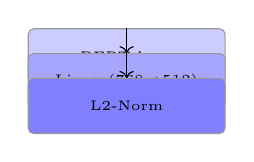
\begin{tikzpicture}[scale=0.45]
      \node[innerarch,fill=blue!20,minimum width=2.5cm] (bert) at (0,0.6) {BERT-base};
      \node[innerarch,fill=blue!35,minimum width=2.5cm] (proj) at (0,-0.1) {Linear(768$\to$512)};
      \node[innerarch,fill=blue!50,minimum width=2.5cm] (norm) at (0,-0.8) {L2-Norm};
      \draw[->] (bert)--(proj); \draw[->](proj)--(norm);
    \end{tikzpicture}\\[2pt]
    $e_t = \frac{W_t \bar{h}}{\|W_t \bar{h}\|_2}$
  };

  \node[modelbox, right=1.5cm of imgq, minimum height=2.8cm, text width=3.2cm] (imgenc) {
    \textbf{ImageEncoder}\\
    (ResNet-50 + Proj)\\[2pt]
    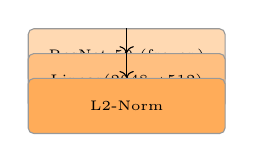
\begin{tikzpicture}[scale=0.45]
      \node[innerarch,fill=orange!30,minimum width=2.5cm] (res) at (0,0.6) {ResNet-50 (frozen)};
      \node[innerarch,fill=orange!50,minimum width=2.5cm] (iproj) at (0,-0.1) {Linear(2048$\to$512)};
      \node[innerarch,fill=orange!65,minimum width=2.5cm] (inorm) at (0,-0.8) {L2-Norm};
      \draw[->](res)--(iproj); \draw[->](iproj)--(inorm);
    \end{tikzpicture}\\[2pt]
    $e_v = \frac{W_v \phi(x_v)}{\|W_v \phi(x_v)\|_2}$
  };

  \node[modelbox, right=1.5cm of audq, minimum height=2.8cm, text width=3.2cm] (audenc) {
    \textbf{AudioEncoder}\\
    (Wav2Vec 2.0 + Proj)\\[2pt]
    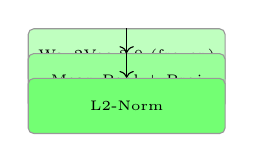
\begin{tikzpicture}[scale=0.45]
      \node[innerarch,fill=green!25,minimum width=2.5cm] (wav) at (0,0.6) {Wav2Vec 2.0 (frozen)};
      \node[innerarch,fill=green!40,minimum width=2.5cm] (aproj) at (0,-0.1) {Mean-Pool + Proj};
      \node[innerarch,fill=green!55,minimum width=2.5cm] (anorm) at (0,-0.8) {L2-Norm};
      \draw[->](wav)--(aproj); \draw[->](aproj)--(anorm);
    \end{tikzpicture}\\[2pt]
    $e_a = \frac{\bar{h}^{(12)}}{\|\bar{h}^{(12)}\|_2}$
  };

  % ── FUSION ────────────────────────────────────────────────
  \node[modelbox, right=1.5cm of textenc, yshift=-2.2cm,
        minimum height=2.0cm, text width=3cm] (fusion) {
    \textbf{Multimodal}\\
    \textbf{Fusion}\\[3pt]
    $e_q = \frac{e_t + e_v + e_a}{3}$\\
    $e_q \in \mathcal{S}^{511}$
  };

  % ── DOMAIN CONFIG ─────────────────────────────────────────
  \node[basebox, fill=lightgraybox, right=1.5cm of fusion,
        yshift=0.8cm, text width=3cm, minimum height=1.6cm] (domain) {
    \textbf{Domain Config}\\[3pt]
    $D \in \{D_{\text{gen}}, D_{\text{med}}\}$\\
    \texttt{hint(q)} $\to$ auto-swap
  };

  % ── FAISS DENSE RETRIEVAL ─────────────────────────────────
  \node[modelbox, below=0.8cm of domain, text width=3cm, minimum height=1.8cm] (faiss) {
    \textbf{FAISS Dense}\\
    \textbf{Retrieval}\\[3pt]
    $\text{top-}K = \underset{d \in \mathcal{I}}{\arg\!\max}_K\; e_q \cdot e_d$\\
    $K=20$
  };

  % ── KG RERANKER ───────────────────────────────────────────
  \node[modelbox, below=0.8cm of faiss, text width=3cm, minimum height=2.0cm] (kgrerank) {
    \textbf{KG Reranker}\\[3pt]
    $s_f = \alpha s_d + (1{-}\alpha)\beta$\\
    $\alpha = 0.6$\\
    $\text{top-}N = 5$
  };

  % ── CONFIDENCE TIER ───────────────────────────────────────
  \node[decisionbox, below=1.0cm of kgrerank, text width=2.6cm] (confcheck) {
    $c = \max s_f$\\
    $c \geq \tau_D$?
  };

  % ── REJECTED ──────────────────────────────────────────────
  \node[resultbox, left=1.5cm of confcheck, yshift=-0.4cm] (rejected) {
    \textbf{REJECTED}\\
    \texttt{answer = ""}\\
    \texttt{confidence}\\
    \texttt{= "rejected"}
  };

  % ── LLM GENERATOR ─────────────────────────────────────────
  \node[modelbox, below=1.0cm of confcheck, text width=3.2cm, minimum height=1.8cm] (llmgen) {
    \textbf{LLM Generator}\\
    (Groq / Llama-3.1-8B)\\[3pt]
    RAG prompt + top-$N$ docs\\
    $\to$ \texttt{answer}
  };

  % ── GENERATOR OUTPUT ──────────────────────────────────────
  \node[reportbox, below=0.8cm of llmgen, minimum height=1.6cm] (genout) {
    \textbf{GeneratorOutput}\\[3pt]
    \texttt{answer}, \texttt{sources}\\
    \texttt{confidence\_level}\\
    \texttt{rejected}
  };

  % ── TEST RUNNER (right column) ────────────────────────────
  \node[suitebox, right=1.8cm of domain, yshift=0.6cm, minimum height=1.4cm] (s1) {
    \textbf{Suite 1}\\Unit Tests\\(11 tests)
  };
  \node[suitebox, below=0.5cm of s1] (s2) {
    \textbf{Suite 2}\\Integration\\(6 tests)
  };
  \node[suitebox, below=0.5cm of s2] (s3) {
    \textbf{Suite 3}\\Domain Swap\\(6 tests)
  };
  \node[suitebox, below=0.5cm of s3] (s4) {
    \textbf{Suite 4}\\Confidence\\(5 tests)
  };
  \node[suitebox, below=0.5cm of s4] (s5) {
    \textbf{Suite 5}\\Retrieval Eval\\(5 tests)
  };
  \node[suitebox, below=0.5cm of s5] (s6) {
    \textbf{Suite 6}\\Regression\\(5 tests)
  };

  % ── REPORT OUTPUT ─────────────────────────────────────────
  \node[reportbox, below=0.5cm of s6] (report) {
    \textbf{test\_report.json}\\
    $\text{pass\_rate} \in [0,100\%]$\\
    P@1, P@3, MRR, latency
  };

  % ── ARROWS: inputs → encoders ─────────────────────────────
  \draw[thickarrow] (textq.east) -- (textenc.west);
  \draw[thickarrow] (imgq.east)  -- (imgenc.west);
  \draw[thickarrow] (audq.east)  -- (audenc.west);

  % ── ARROWS: encoders → fusion ─────────────────────────────
  \draw[thickarrow] (textenc.east) -| ($(fusion.north west)!0.5!(fusion.north)$);
  \draw[thickarrow] (imgenc.east)  --  (fusion.west);
  \draw[thickarrow] (audenc.east)  -| ($(fusion.south west)!0.5!(fusion.south)$);

  % ── ARROWS: pipeline flow ─────────────────────────────────
  \draw[thickarrow] (domain.south)   -- (faiss.north);
  \draw[thickarrow] (faiss.south)    -- (kgrerank.north);
  \draw[thickarrow] (kgrerank.south) -- (confcheck.north);
  \draw[thickarrow] (fusion.east)    -- (domain.west);

  % ── CONFIDENCE BRANCHES ───────────────────────────────────
  \draw[redarrow]   (confcheck.west) -- node[above,font=\tiny]{NO} (rejected.east);
  \draw[greenarrow] (confcheck.south) -- node[right,font=\tiny]{YES} (llmgen.north);
  \draw[thickarrow] (llmgen.south)   -- (genout.north);

  % ── TEST SUITE ARROWS (dashed monitors) ──────────────────
  \draw[dashedarrow,color=accentgreen!70] (genout.east) -| (s2.south);
  \draw[dashedarrow,color=accentgreen!70] (domain.east) -- (s3.west);
  \draw[dashedarrow,color=accentgreen!70] (confcheck.east) -| (s4.west);
  \draw[dashedarrow,color=accentgreen!70] (faiss.east) -- (s5.west);
  \draw[dashedarrow,color=accentgreen!70] (s6.south) -- (report.north);

  % Suite 1 monitors encoders
  \draw[dashedarrow,color=accentgreen!70] (textenc.north) |- ($(s1.west)+(0,0.2)$);

  % ── BACKGROUND CONTAINER ─────────────────────────────────
  \begin{pgfonlayer}{background}
    \node[rectangle, draw=darkbluecontainer, fill=darkbluecontainer!25,
          very thick, rounded corners=8pt,
          fit=(textq)(audq)(textenc)(audenc)(fusion)(domain)(faiss)(kgrerank)
              (confcheck)(rejected)(llmgen)(genout),
          inner sep=14pt, label={[font=\small\bfseries,color=accentblue]above:
            \textbf{MIVA-KNIGHT Inference Pipeline}}] (maincontainer) {};
    \node[rectangle, draw=accentgreen!60, fill=accentgreen!8,
          thick, rounded corners=6pt,
          fit=(s1)(s2)(s3)(s4)(s5)(s6)(report),
          inner sep=8pt, label={[font=\small\bfseries,color=accentgreen!70!black]above:
            \textbf{MIVATestRunner}}] (testcontainer) {};
  \end{pgfonlayer}

\end{tikzpicture}
}
\caption{Complete MIVA-KNIGHT pipeline architecture with test harness. Blue container:
inference pipeline. Green container: \texttt{MIVATestRunner} with six test suites.
Dashed arrows indicate monitoring / assertion paths.}
\label{fig:full-pipeline}
\end{figure}

\newpage

% =============================================================
%  SECTION 1: EXECUTION CONTRACT & MODULE BOOTSTRAP
% =============================================================
\section{Module Bootstrap \& Execution Contract}
\label{sec:bootstrap}

\subsection{Technical Description}

The \texttt{test\_miva\_knight.py} module establishes a formal \textbf{execution contract}
before any test runs. This contract defines three preconditions:

\begin{mdef}[Execution Preconditions]
Let $\Omega$ denote the Colab runtime environment. The test module requires:
\[
  \text{Preconditions}(\Omega) = \begin{cases}
    \texttt{Cell~2 executed}     & \text{all path variables set in } \Omega \\
    \texttt{pipeline.load()}     & \text{models and indices in memory} \\
    \texttt{GROQ\_API\_KEY} \in \text{env} & \text{optional — generation tests skipped if absent}
  \end{cases}
\]
The Groq availability indicator is:
\[
  \texttt{\_has\_groq} = \mathbf{1}\bigl[\texttt{GROQ\_API\_KEY} \in \text{env}(\Omega)\bigr] \in \{0, 1\}
\]
\end{mdef}

\subsection{Algorithm: Module Bootstrap}

\begin{algorithm}[H]
\caption{Module Bootstrap --- \texttt{test\_miva\_knight.py} initialisation}
\label{alg:bootstrap}
\begin{algorithmic}[1]
\Require Colab runtime $\Omega$ with \texttt{MIVA\_PROJECT\_ROOT} set
\Ensure All classes and functions loaded; no tests executed
\State Import standard library: \texttt{os, sys, json, time, random, traceback, datetime}
\State Import typing: \texttt{List, Dict, Any, Optional, Callable}
\State Import dataclass utilities: \texttt{dataclass, field}
\State Import \texttt{torch}, \texttt{torch.nn.functional as F}
\State Define \texttt{TestResult} dataclass \Comment{7-tuple result record}
\State Define \texttt{SuiteResult} dataclass \Comment{suite-level aggregator}
\State Define \texttt{MIVATestRunner} class \Comment{orchestrates all 6 suites}
\State Define \texttt{run\_tests()} convenience function
\end{algorithmic}
\end{algorithm}

\begin{plainbox}
Think of this step as unpacking a toolbox before starting work. Every tool
(library) needed to measure, time, log, and compare test results is loaded here.
Nothing runs yet --- it is pure setup. Like a chef laying out all their knives
and measuring cups before cooking starts.
\end{plainbox}

\newpage

% =============================================================
%  SECTION 2: RESULT DATA STRUCTURES
% =============================================================
\section{Result Data Structures: \texttt{TestResult} \& \texttt{SuiteResult}}
\label{sec:datastructs}

\subsection{Formal Definitions}

\begin{mdef}[TestResult]
A \texttt{TestResult} is a 7-tuple:
\[
  r = \bigl(\,\text{name},\;\text{suite},\;p,\;\Delta t,\;\text{detail},\;v,\;\text{err}\,\bigr)
\]
where the components are:
\begin{align*}
  \text{name}   &\in \Sigma^* && \text{human-readable test identifier} \\
  \text{suite}  &\in \Sigma^* && \text{parent suite name} \\
  p             &\in \{\text{True},\text{False}\} && \text{pass/fail boolean} \\
  \Delta t      &\in \mathbb{R}_{\geq 0} && \text{wall-clock duration (seconds)} \\
  \text{detail} &\in \Sigma^* && \text{human-readable result summary} \\
  v             &\in \mathbb{R} \cup \{\texttt{None}\} && \text{numeric value if applicable} \\
  \text{err}    &\in \Sigma^* && \text{traceback string (empty if } p = \text{True}\text{)}
\end{align*}
\end{mdef}

\begin{mdef}[SuiteResult]
A \texttt{SuiteResult} aggregates all \texttt{TestResult} records for a named suite:
\[
  S = \bigl(\,\text{name},\;\text{passed},\;\text{failed},\;\text{skipped},\;
            [r_1, r_2, \ldots, r_n]\,\bigr)
\]
with two computed properties:
\[
  \text{total}(S) = |\text{passed}| + |\text{failed}| + |\text{skipped}|
\]
\[
  \text{pass\_rate}(S) = \frac{|\text{passed}|}{\max\!\bigl(\text{total}(S),\,1\bigr)} \times 100\%
\]
\end{mdef}

\begin{mlemma}[Pass-Rate Bounds]
For any \texttt{SuiteResult} $S$:
\[
  0 \;\leq\; \text{pass\_rate}(S) \;\leq\; 100\%
\]
\textit{Proof.} The numerator $|\text{passed}| \geq 0$ and the denominator
$\max(\text{total}(S), 1) \geq 1$, so the ratio lies in $[0, 1]$.
Multiplied by $100$ the result lies in $[0, 100]$. \hfill$\square$
\end{mlemma}

\subsection{Data Flow Flowchart}

\begin{figure}[H]
\centering
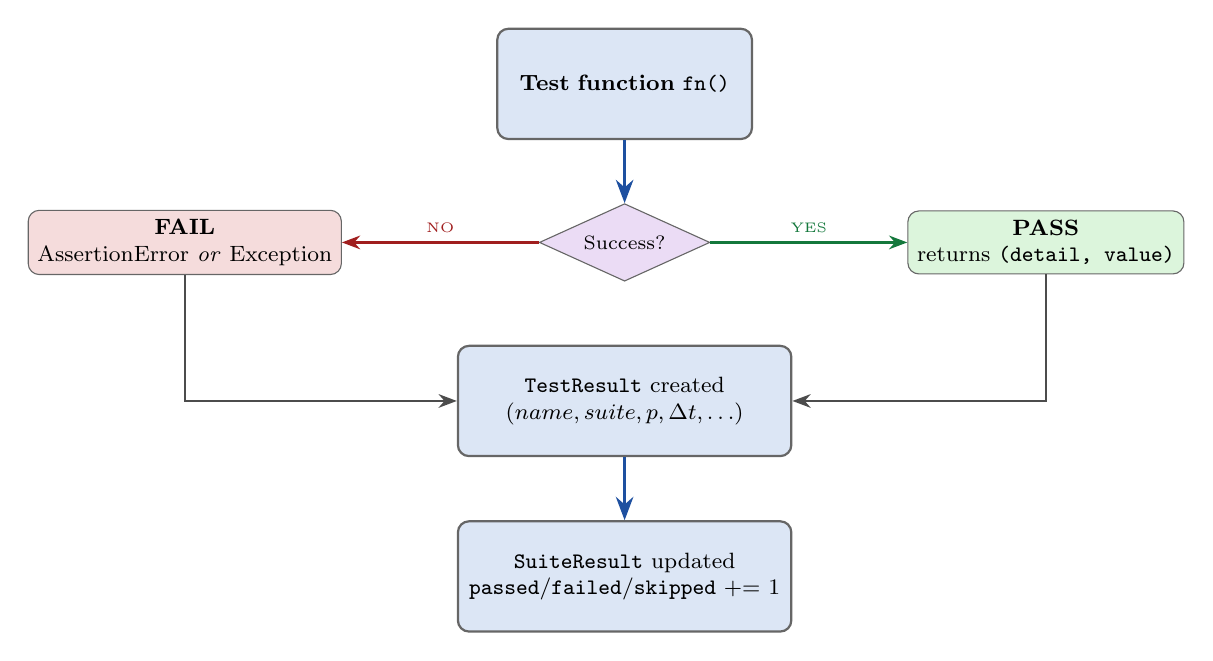
\begin{tikzpicture}[node distance=0.9cm and 1.5cm]
  \node[modelbox, text width=3cm] (fn) {\textbf{Test function} \texttt{fn()}};
  \node[decisionbox, below=0.8cm of fn] (outcome) {Success?};
  \node[basebox, fill=lightgreenbox, right=2.5cm of outcome, minimum width=3.2cm] (pass)
        {\textbf{PASS}\\returns \texttt{(detail, value)}};
  \node[basebox, fill=lightredbox, left=2.5cm of outcome, minimum width=3.2cm] (fail)
        {\textbf{FAIL}\\AssertionError \textit{or} Exception};
  \node[modelbox, below=0.8cm of outcome, text width=4cm] (result)
        {\texttt{TestResult} created\\$(name, suite, p, \Delta t, \ldots)$};
  \node[modelbox, below=0.8cm of result, text width=4cm] (suite)
        {\texttt{SuiteResult} updated\\\texttt{passed}/\texttt{failed}/\texttt{skipped} += 1};

  \draw[thickarrow] (fn) -- (outcome);
  \draw[greenarrow] (outcome.east) -- node[above,font=\tiny]{YES} (pass.west);
  \draw[redarrow]   (outcome.west) -- node[above,font=\tiny]{NO}  (fail.east);
  \draw[arrow] (pass.south) |- (result.east);
  \draw[arrow] (fail.south) |- (result.west);
  \draw[thickarrow] (result) -- (suite);
\end{tikzpicture}
\caption{Data flow from test function through \texttt{TestResult} to \texttt{SuiteResult}.}
\label{fig:result-flow}
\end{figure}

\begin{plainbox}
\texttt{TestResult} is like a report card entry for a single exam question:
did it pass, how long did it take, and if it failed --- what went wrong?
\texttt{SuiteResult} is the full report card for one subject (e.g.\ ``Unit Tests''),
showing a final percentage score. The \texttt{pass\_rate} formula ensures you can never
get below 0\% or above 100\%, even if something unexpected happens.
\end{plainbox}

\newpage

% =============================================================
%  SECTION 3: MIVA TEST RUNNER — CONSTRUCTOR & _run HELPER
% =============================================================
\section{\texttt{MIVATestRunner}: Constructor \& Universal Test Executor}
\label{sec:testrunner}

\subsection{Constructor Specification}

\begin{mdef}[Runner Configuration]
\texttt{MIVATestRunner.\_\_init\_\_} stores the runner configuration tuple:
\[
  \mathcal{R} = \bigl(\texttt{pipeline},\;\texttt{roco\_val},\;\texttt{coco\_meta},\;
                n_{\text{eval}},\;s_{\text{seed}}\bigr)
\]
and initialises an empty result registry:
\[
  \texttt{\_results} : \text{suiteName} \;\mapsto\; \texttt{SuiteResult} \quad
  \bigl(\text{initially } \emptyset\bigr)
\]
The Groq availability flag:
\[
  \texttt{\_has\_groq} = \mathbf{1}\bigl[\texttt{GROQ\_API\_KEY} \in \text{env}\bigr]
\]
\end{mdef}

\subsection{The Universal Test Executor: \texttt{\_run}}

Every one of the 38 individual tests in MIVA-KNIGHT passes through a single method,
\texttt{\_run}, which acts as a universal referee.

\begin{algorithm}[H]
\caption{\texttt{\_run(suite, name, fn, skip\_if, skip\_reason)} --- Universal test executor}
\label{alg:run}
\begin{algorithmic}[1]
\Require Suite name \textit{suite}, test name \textit{name}, callable \textit{fn},
         boolean \textit{skip\_if}, string \textit{skip\_reason}
\Ensure \texttt{TestResult} $r$ appended to \texttt{SuiteResult}; no crash propagation

\If{\textit{suite} $\notin$ \texttt{\_results}}
  \State $\texttt{\_results}[\text{suite}] \gets \texttt{SuiteResult}(\text{name}=\text{suite})$
\EndIf
\State $sr \gets \texttt{\_results}[\text{suite}]$

\vspace{4pt}
\Comment{--- Skip path ---}
\If{\textit{skip\_if} $= \text{True}$}
  \State $r \gets \texttt{TestResult}(\text{passed}=\text{False},\;\text{detail}=\texttt{"SKIP: "} + \text{skip\_reason})$
  \State $sr.\text{skipped} \mathrel{+}= 1$
  \State Print \texttt{[SKIP] name  (skip\_reason)}
  \State \Return $r$
\EndIf

\vspace{4pt}
\Comment{--- Execute path ---}
\State $t_0 \gets \text{wall-clock time}$
\State \textbf{try:}
\State \quad $(\text{detail},\;v) \gets fn()$ \Comment{Call the actual test function}
\State \quad $p \gets \text{True}$;\quad $\text{err} \gets \texttt{""}$
\State \textbf{except AssertionError} $e$\textbf{:}
\State \quad $p \gets \text{False}$;\quad $\text{detail} \gets \text{str}(e)$;\quad $v \gets \texttt{None}$
\State \quad $\text{err} \gets \texttt{""}$ \Comment{Expected failure --- no traceback needed}
\State \textbf{except Exception} $e$\textbf{:}
\State \quad $p \gets \text{False}$;\quad $\text{detail} \gets \text{str}(e)$;\quad $v \gets \texttt{None}$
\State \quad $\text{err} \gets \texttt{format\_traceback()}$ \Comment{Unexpected --- capture full trace}

\vspace{4pt}
\Comment{--- Record ---}
\State $\Delta t \gets \text{wall-clock} - t_0$
\State $r \gets \texttt{TestResult}(\text{name},\;\text{suite},\;p,\;\Delta t,\;\text{detail},\;v,\;\text{err})$
\If{$p = \text{True}$}
  \State $sr.\text{passed} \mathrel{+}= 1$;\quad Print \texttt{[PASS] name (}$\Delta t$\texttt{s) detail}
\Else
  \State $sr.\text{failed} \mathrel{+}= 1$;\quad Print \texttt{[FAIL] name (}$\Delta t$\texttt{s) detail}
  \If{$\text{err} \neq \texttt{""}$} Print last line of traceback \EndIf
\EndIf
\State $sr.\text{results.append}(r)$
\State \Return $r$
\end{algorithmic}
\end{algorithm}

\begin{mtheorem}[Exception Isolation]
For any test function $f_i$ in a suite, an uncaught exception inside $f_i$
does \emph{not} abort subsequent tests $f_{i+1}, f_{i+2}, \ldots$ in the same suite.

\textit{Proof.} The \texttt{try/except} block in \texttt{\_run} catches both
\texttt{AssertionError} (expected test failure) and the base \texttt{Exception}
class (unexpected runtime error). In both branches, control unconditionally
proceeds to the \texttt{TestResult} construction and
\texttt{sr.results.append(r)} statements, returning normally to the calling
loop. Since the loop iterates over a fixed sequence of \texttt{\_run} calls,
no call can prevent subsequent calls from executing. \hfill$\square$
\end{mtheorem}

\subsection{\texttt{\_run} Control Flow Diagram}

\begin{figure}[H]
\centering
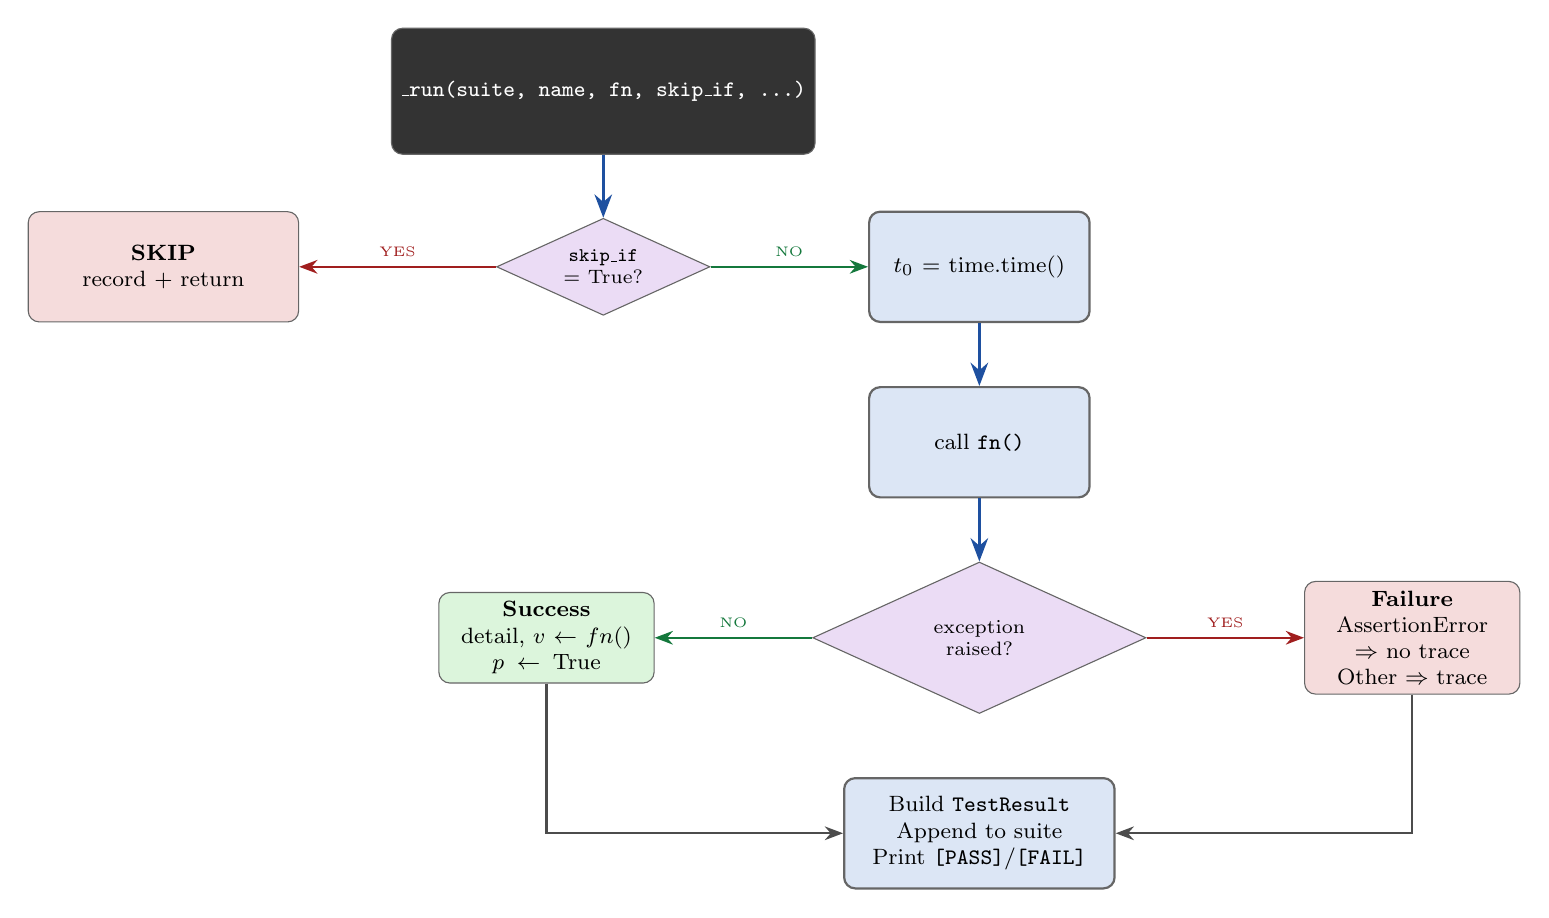
\begin{tikzpicture}[node distance=0.85cm and 2cm]
  \node[inputbox] (entry) {\texttt{\_run(suite, name, fn, skip\_if, ...)}};
  \node[decisionbox, below=0.8cm of entry] (skipq) {\texttt{skip\_if}\\= True?};
  \node[resultbox, left=2.5cm of skipq] (skipnode) {\textbf{SKIP}\\record + return};
  \node[modelbox, right=2.0cm of skipq, text width=2.5cm] (timer) {$t_0 = \text{time.time()}$};
  \node[modelbox, below=0.8cm of timer, text width=2.5cm] (callfn) {call \texttt{fn()}};
  \node[decisionbox, below=0.8cm of callfn, text width=2.5cm] (excq) {exception\\raised?};
  \node[basebox, fill=lightgreenbox, left=2cm of excq, text width=2.5cm] (success)
        {\textbf{Success}\\$\text{detail, } v \gets fn()$\\$p \gets \text{True}$};
  \node[basebox, fill=lightredbox, right=2cm of excq, text width=2.5cm] (fail)
        {\textbf{Failure}\\AssertionError\\$\Rightarrow$ no trace\\Other $\Rightarrow$ trace};
  \node[modelbox, below=0.8cm of excq, text width=3.2cm] (record)
        {Build \texttt{TestResult}\\Append to suite\\Print \texttt{[PASS]}/\texttt{[FAIL]}};

  \draw[thickarrow] (entry)  -- (skipq);
  \draw[redarrow]   (skipq.west) -- node[above,font=\tiny]{YES} (skipnode.east);
  \draw[greenarrow] (skipq.east) -- node[above,font=\tiny]{NO} (timer.west);
  \draw[thickarrow] (timer)  -- (callfn);
  \draw[thickarrow] (callfn) -- (excq);
  \draw[greenarrow] (excq.west) -- node[above,font=\tiny]{NO} (success.east);
  \draw[redarrow]   (excq.east) -- node[above,font=\tiny]{YES} (fail.west);
  \draw[arrow] (success.south) |- (record.west);
  \draw[arrow] (fail.south)    |- (record.east);
\end{tikzpicture}
\caption{\texttt{\_run} internal control flow. Every path leads to a \texttt{TestResult} record.}
\label{fig:run-flow}
\end{figure}

\begin{plainbox}
\texttt{\_run} is the referee for every single test. It starts a stopwatch, calls the
test, and catches any crash --- recording pass/fail and timing regardless of what
happens inside. Skipping is handled cleanly upfront so optional tests (like ones
needing a Groq API key) never cause noise. The key insight: \emph{no single test can
break the whole test run}.
\end{plainbox}

\newpage

% =============================================================
%  SECTION 4: SUITE 1 — UNIT TESTS
% =============================================================
\section{Suite 1: Unit Tests (11 Tests)}
\label{sec:unit}

Unit tests verify each \textbf{component in isolation} --- no end-to-end pipeline,
no LLM, no disk I/O beyond what the component itself requires.

\begin{mdef}[Unit Test Scope]
A unit test $u_i$ is a function that exercises a \emph{single} component
$\mathcal{C}_i$ with a fixed, known input and asserts a deterministic property:
\[
  u_i: \mathcal{C}_i \;\times\; x_i^{\text{fixed}} \;\to\; \{\text{PASS}, \text{FAIL}\}
\]
No inter-component data flows are tested within a unit test.
\end{mdef}

\subsection{Test 1.1 — TextEncoder Output Shape}

\begin{mdef}[Text Encoder Map]
The text encoder is a function:
\[
  f_{\text{text}}: \Sigma^* \;\longrightarrow\; \mathbb{R}^{512}
\]
mapping an arbitrary string query $q$ to a 512-dimensional real vector.
\end{mdef}

\textbf{Assertion:}
\[
  \texttt{out.text\_emb.shape} = (512,) \;\land\; \texttt{out.text\_emb.dtype} = \texttt{float32}
\]

\begin{plainbox}
Check that the encoder's output is exactly a 512-number vector --- not 256, not 1024.
Like verifying a standard plug fits a standard socket. If the shape is wrong,
nothing downstream will work.
\end{plainbox}

\subsection{Test 1.2 — TextEncoder L2 Norm}

\begin{mdef}[Unit-Normalised Embedding]
An embedding $e \in \mathbb{R}^{512}$ is \emph{unit-normalised} (lies on the unit sphere
$\mathcal{S}^{511}$) if and only if:
\[
  \|e\|_2 = \sqrt{\sum_{i=1}^{512} e_i^2} = 1.0
\]
\end{mdef}

\textbf{Assertion} (with numerical tolerance $\varepsilon = 0.01$):
\[
  \bigl|\,\|e\|_2 - 1.0\,\bigr| < 0.01
\]

\begin{mlemma}[Cosine Equivalence on Unit Sphere]
For two unit-normalised embeddings $u, v \in \mathcal{S}^{511}$:
\[
  \cos(u, v) \;=\; \frac{u \cdot v}{\|u\|_2\|v\|_2} \;=\; u \cdot v
\]
Therefore, FAISS inner-product search is equivalent to cosine similarity search
\textit{if and only if} all stored embeddings are L2-normalised.

\textit{Proof.} By definition of cosine similarity and $\|u\|_2 = \|v\|_2 = 1$,
the denominator equals $1$. \hfill$\square$
\end{mlemma}

\begin{plainbox}
The embedding must be a unit vector --- its ``length'' must be exactly 1.0.
If it is not, every similarity score in the system will be wrong.
Think of it like a compass needle: it only points correctly if it has the right length.
A compass with a needle 2$\times$ too long or too short still spins but gives
misleading readings.
\end{plainbox}

\subsection{Test 1.3 — TextEncoder NER Entities}

\begin{mdef}[Named Entity Recognition Function]
The NER component maps a string to a set of extracted entity strings:
\[
  \text{NER}: \Sigma^* \;\to\; 2^{\mathcal{E}}
\]
where $\mathcal{E}$ is the vocabulary of recognised entity types.
\end{mdef}

\textbf{Assertion:}
\[
  \texttt{isinstance(out.entities, list)} = \text{True}
  \;\land\;
  |\texttt{out.entities}| > 0
\]

\begin{plainbox}
Feed ``a dog running on a sandy beach'' and get back a non-empty list like
\texttt{['dog', 'beach']}. The Knowledge Graph re-ranker needs these to find
related concepts and boost retrieval scores. If NER returns nothing, the KG
re-ranker is blind.
\end{plainbox}

\subsection{Tests 1.4 \& 1.5 — Medical Domain Hint}

\begin{mdef}[Domain Hint Function]
\[
  \text{hint}(q) = \begin{cases}
    \texttt{"medical"} & \text{if } q \text{ contains medical keywords from a whitelist} \\
    \texttt{None}      & \text{otherwise}
  \end{cases}
\]
\end{mdef}

\textbf{Test 1.4 --- True Positive:}
\[
  \text{hint}(\text{``bilateral pneumonia with pleural effusion''}) = \texttt{"medical"}
\]

\textbf{Test 1.5 --- True Negative:}
\[
  \text{hint}(\text{``a dog running on a beach''}) = \texttt{None}
\]

\begin{mlemma}[Hint Precision and Recall on Probe Set]
Tests 1.4 and 1.5 together assert on the two-sample probe set
$\{q_{\text{med}}, q_{\text{gen}}\}$:
\[
  \text{Precision} = \frac{\text{TP}}{\text{TP}+\text{FP}} = \frac{1}{1} = 1
  \qquad
  \text{Recall} = \frac{\text{TP}}{\text{TP}+\text{FN}} = \frac{1}{1} = 1
\]
where $\text{TP}=1$ (medical query correctly flagged) and $\text{FP}=0$
(general query not spuriously flagged). \hfill$\square$
\end{mlemma}

\begin{plainbox}
Test 1.4 checks the ``medical alarm'' fires for a chest-scan query.
Test 1.5 checks the alarm does NOT fire for a dog photo.
This matters because a spurious medical hint triggers an expensive index swap
from COCO (5\,000 docs) to ROCO (65\,000 docs) --- and that takes time.
\end{plainbox}

\subsection{Test 1.6 — Embedding Distinctness}

\begin{mdef}[Embedding Collapse]
A projection head is \emph{collapsed} if:
\[
  \forall\, q_1, q_2 \in \Sigma^*:\;\;
  \cos\!\bigl(f(q_1),\, f(q_2)\bigr) \approx 1.0
\]
i.e., all queries map to nearly the same point on $\mathcal{S}^{511}$.
\end{mdef}

\textbf{Assertion (anti-collapse check):}
\[
  \cos\!\Bigl(f\bigl(\text{``a dog on a beach''}\bigr),\;
              f\bigl(\text{``chest X-ray showing cardiomegaly''}\bigr)\Bigr) < 0.95
\]

\begin{plainbox}
Two completely different queries (a dog photo vs.\ a medical scan) must produce
meaningfully different 512-dimensional vectors. If they are 99\% similar, the model
has ``collapsed'' --- it cannot distinguish anything and will return the same results
for every query, regardless of content.
\end{plainbox}

\subsection{Test 1.7 — Emotion Centroids Shape}

\begin{mdef}[Emotion Centroid Matrix]
Let $\mathcal{E}_8 = \{e_1, \ldots, e_8\}$ be the 8 RAVDESS emotions
(neutral, calm, happy, sad, angry, fearful, disgust, surprised).
The centroid matrix is:
\[
  C \in \mathbb{R}^{8 \times 512}, \qquad
  C_i = \frac{1}{|\mathcal{A}_i|}\sum_{a \in \mathcal{A}_i} \text{AudioEncoder}(a)
\]
where $\mathcal{A}_i$ is the set of audio clips for emotion $i$.
\end{mdef}

\textbf{Assertions:}
\[
  C.\text{shape} = (8, 512) \;\land\;
  \forall i \in \{1,\ldots,8\}:\;\|C_i\|_2 > 0.01
\]

\begin{plainbox}
Check there is one learned average audio fingerprint per emotion, and none are
all-zeros (which would mean that emotion was never seen during training, or the
centroid was never computed). An all-zero centroid would make every audio query
appear equidistant from that emotion.
\end{plainbox}

\subsection{Tests 1.8 \& 1.9 — FAISS Index and Knowledge Graph}

\begin{mdef}[FAISS Dense Index]
The dense index stores $N$ document embeddings:
\[
  \mathcal{I} = \{(d_j, e_j)\}_{j=1}^{N}, \qquad e_j \in \mathcal{S}^{511}
\]
\textbf{Test 1.8 Assertion:} $\mathcal{I} \neq \texttt{None} \;\land\; N > 0$
\end{mdef}

\begin{mdef}[Knowledge Graph]
$\mathcal{G} = (\mathcal{V}, \mathcal{E}, \mathcal{R})$ stored as a Python dict
keyed by entity strings.\\
\textbf{Test 1.9 Assertion:} $\mathcal{G} \neq \texttt{None} \;\land\; |\mathcal{G}| > 0$
\end{mdef}

\subsection{Tests 1.10 \& 1.11 — Domain Config File Paths}

\begin{mdef}[Domain Configuration Contract]
Each domain object $D$ must expose three resolvable file paths:
\[
  \text{DomainContract}(D) = \bigl\{p_{\text{FAISS}},\; p_{\text{corpus}},\; p_{\text{KG}}\bigr\}
\]
\textbf{Assertion (both GeneralDomain and MedicalDomain):}
\[
  \forall p \in \text{DomainContract}(D):\; \texttt{os.path.exists}(p) = \text{True}
\]
\end{mdef}

\subsection{Suite 1 Algorithm}

\begin{algorithm}[H]
\caption{\texttt{run\_unit()} --- 11 component isolation tests}
\label{alg:unit}
\begin{algorithmic}[1]
\Require \texttt{pipeline} loaded with all encoders, retriever, and domain config
\Ensure 11 \texttt{TestResult} records appended to \texttt{\_results["unit"]}
\State $p \gets \texttt{self.pipeline}$
\State \Call{\_run}{"unit", "TextEncoder output shape", $\lambda$: assert shape $(512,)$, dtype float32}
\State \Call{\_run}{"unit", "TextEncoder L2 norm", $\lambda$: assert $|\,\|e\|_2 - 1| < 0.01$}
\State \Call{\_run}{"unit", "TextEncoder NER entities", $\lambda$: assert $|\texttt{entities}| > 0$}
\State \Call{\_run}{"unit", "TextEncoder medical domain hint", $\lambda$: assert hint $=$ "medical"}
\State \Call{\_run}{"unit", "TextEncoder no false medical hint", $\lambda$: assert hint $=$ None}
\State \Call{\_run}{"unit", "Embedding distinctness", $\lambda$: assert $\cos(e_1, e_2) < 0.95$}
\State \Call{\_run}{"unit", "AudioEncoder emotion centroids", $\lambda$: assert shape $(8,512)$, no zeros}
\State \Call{\_run}{"unit", "FAISS index loaded", $\lambda$: assert ntotal $> 0$}
\State \Call{\_run}{"unit", "KG loaded", $\lambda$: assert $|\mathcal{G}| > 0$}
\State \Call{\_run}{"unit", "GeneralDomain paths exist", $\lambda$: assert 3 paths exist}
\State \Call{\_run}{"unit", "MedicalDomain paths exist", $\lambda$: assert 3 paths exist}
\State \Return \texttt{\_results["unit"]}
\end{algorithmic}
\end{algorithm}

\begin{plainbox}[Suite 1 Summary]
Suite 1 is a pre-flight checklist. Before anything runs end-to-end, we verify every
individual component loaded correctly and produces sensible outputs on a known input.
Like a pilot checking each instrument separately before taking off --- not flying
anywhere yet, just confirming every gauge works.
\end{plainbox}

\newpage

% =============================================================
%  SECTION 5: SUITE 2 — INTEGRATION TESTS
% =============================================================
\section{Suite 2: Integration Tests (6 Tests)}
\label{sec:integration}

Integration tests verify that \textbf{components work together} as a system. The
complete data path under test is:
\[
  \text{TextQuery}(q)
  \;\xrightarrow{f_{\text{text}}}\; e_q
  \;\xrightarrow{\text{FAISS}}\; \text{docs}
  \;\xrightarrow{\text{KG rerank}}\; \text{top-}N
  \;\xrightarrow{\text{generator}}\; \text{GeneratorOutput}
\]

\subsection{Test 2.1 — Pipeline Returns \texttt{GeneratorOutput}}

\begin{mdef}[GeneratorOutput Contract]
The pipeline's \texttt{query(q)} method must return an object $r$ satisfying:
\[
  \texttt{isinstance}(r,\;\texttt{GeneratorOutput})
  \;\land\;
  \bigl\{\texttt{confidence\_level},\;\texttt{sources},\;\texttt{rejected}\bigr\} \subseteq \text{attrs}(r)
\]
\end{mdef}

\subsection{Test 2.2 — Sources Populated on Non-Rejected Result}

\begin{mdef}[RAG Grounding Contract]
If the pipeline does not reject a query, the returned sources must be non-empty:
\[
  \neg\,\text{rejected} \;\Rightarrow\; |\text{sources}| > 0
\]
This is the \emph{Retrieval-Augmented Generation (RAG) contract}: every confident
answer must be grounded in retrieved documents.
\end{mdef}

\begin{maxiom}[RAG Grounding]
An answer generated without retrieved sources is an ungrounded hallucination and
must not be returned to the user.
\end{maxiom}

\subsection{Test 2.3 — Rejected Query Produces No Answer}

\begin{mdef}[Rejection Contract]
\[
  \text{rejected} = \text{True} \;\Rightarrow\; \text{answer} \in \{\texttt{""}, \texttt{None}\}
\]
\end{mdef}

Test input: \texttt{"xyzzy qwerty flurble blorb"} --- tokens with no semantic
representation in the embedding space, expected to score below threshold $\tau$.

\subsection{Test 2.4 — Retriever Returns Sorted Top-K Documents}

\begin{mdef}[Dense Retrieval]
Given a query embedding $e_q \in \mathcal{S}^{511}$ and index $\mathcal{I}$:
\[
  \text{DenseSearch}(e_q, K) = \underset{d \in \mathcal{I}}{\text{top-}K}\;\cos(e_q, e_d)
\]
\end{mdef}

\textbf{Assertions:}
\[
  |\text{docs}| = 20
  \;\land\;
  \forall d:\; d\text{ has }\texttt{dense\_score}
  \;\land\;
  s_1 \geq s_2 \geq \cdots \geq s_{20}
\]

\subsection{Test 2.5 — KG Reranker Returns Top-N}

\begin{mdef}[Hybrid Score with KG Boost]
For a document $d$ and query entities $\mathcal{E}_q$:
\begin{align*}
  s_{\text{final}}(d) &= \alpha \cdot s_{\text{dense}}(d) + (1 - \alpha) \cdot \text{GraphBoost}(d, \mathcal{E}_q)\\[4pt]
  \text{GraphBoost}(d, \mathcal{E}_q) &= \min\!\left(1,\;\max_{e \in \mathcal{E}_q}
    \max_{\substack{(\cdot,\cdot,n,h) \in \\ \mathcal{G}.\text{Nbrs}(e,2)}}
    \frac{\mathbf{1}[n \in d]}{h + 1}\right)
\end{align*}
where $h$ is the hop distance, $\alpha = 0.6$, and $\mathcal{G}.\text{Nbrs}(e, 2)$
denotes the 2-hop neighbourhood of entity $e$ in $\mathcal{G}$.
\end{mdef}

\textbf{Assertions:}
\[
  |\text{reranked}| \leq 5 \;\land\; \forall d \in \text{reranked}:\; d\text{ has }\texttt{final\_score}
\]

\begin{mlemma}[Hybrid Score Bounds]
For $\alpha = 0.6$, $s_{\text{dense}} \in [-1, 1]$, and $\text{GraphBoost} \in [0, 1]$:
\[
  s_{\text{final}} \in [-0.6,\; 0.6 + 0.4] = [-0.6,\; 1.0]
\]
\textit{Proof.} Lower bound: $0.6 \cdot (-1) + 0.4 \cdot 0 = -0.6$.
Upper bound: $0.6 \cdot 1 + 0.4 \cdot 1 = 1.0$. \hfill$\square$
\end{mlemma}

\subsection{Test 2.6 — LLM Generation (Optional)}

\begin{mdef}[Generation Condition]
Test 2.6 is skipped when $\texttt{\_has\_groq} = 0$. When active:
\[
  \neg\,\text{rejected} \;\land\; |\text{answer}| > 10 \;\text{characters}
\]
\end{mdef}

\subsection{Suite 2 Algorithm and Flowchart}

\begin{algorithm}[H]
\caption{\texttt{run\_integration()} --- Full pipeline end-to-end tests}
\label{alg:integration}
\begin{algorithmic}[1]
\Require \texttt{pipeline} loaded and responsive
\Ensure 6 \texttt{TestResult} records in \texttt{\_results["integration"]}
\State \Call{\_run}{"integration", "Pipeline returns GeneratorOutput", \ldots}
\State \Call{\_run}{"integration", "Pipeline sources populated", \ldots}
\State \Call{\_run}{"integration", "Rejected query has no answer", \ldots}
\State \Call{\_run}{"integration", "Retriever returns sorted top-K", \ldots}
\State \Call{\_run}{"integration", "KG reranker returns top-N", \ldots}
\State \Call{\_run}{"integration", "LLM generation produces answer", \ldots,
       skip\_if $=\neg\texttt{\_has\_groq}$}
\State \Return \texttt{\_results["integration"]}
\end{algorithmic}
\end{algorithm}

\begin{figure}[H]
\centering
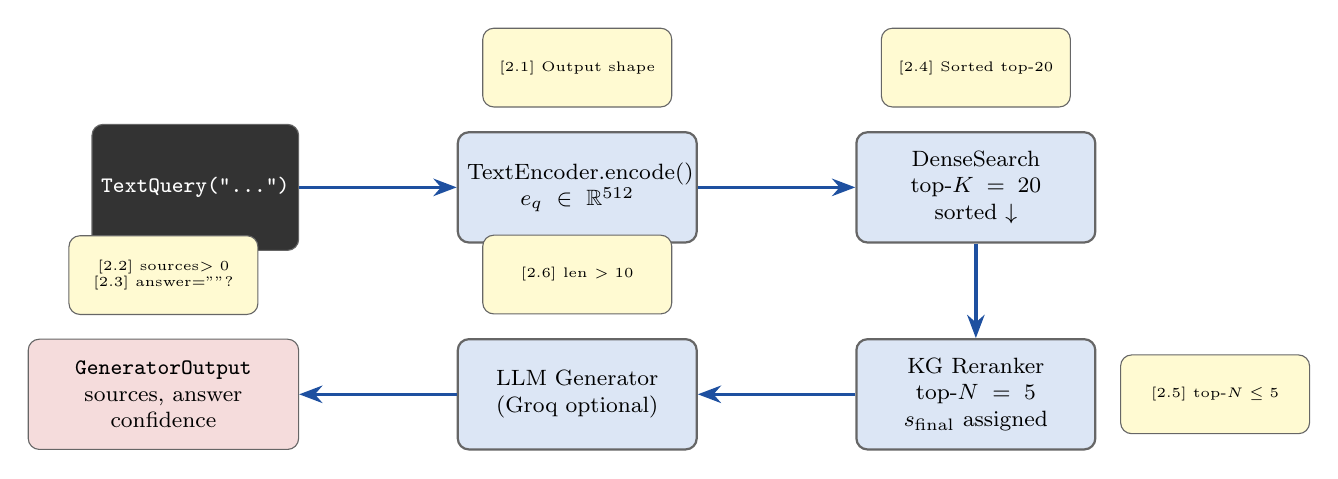
\begin{tikzpicture}[node distance=0.85cm and 1.8cm]
  \node[inputbox] (q) {\texttt{TextQuery("...")}};
  \node[modelbox, right=2cm of q, text width=2.8cm] (enc)
        {TextEncoder.encode()\\$e_q \in \mathbb{R}^{512}$};
  \node[modelbox, right=2cm of enc, text width=2.8cm] (faiss)
        {DenseSearch\\top-$K=20$\\sorted $\downarrow$};
  \node[modelbox, below=1.2cm of faiss, text width=2.8cm] (kg)
        {KG Reranker\\top-$N=5$\\$s_{\text{final}}$ assigned};
  \node[modelbox, left=2cm of kg, text width=2.8cm] (gen)
        {LLM Generator\\(Groq optional)};
  \node[resultbox, left=2cm of gen] (out) {\texttt{GeneratorOutput}\\sources, answer\\confidence};

  % test labels
  \node[testbox, above=0.3cm of enc] {[2.1] Output shape};
  \node[testbox, above=0.3cm of faiss] {[2.4] Sorted top-20};
  \node[testbox, right=0.1cm of kg, xshift=0.2cm] {[2.5] top-$N \leq 5$};
  \node[testbox, above=0.3cm of gen] {[2.6] len $>10$};
  \node[testbox, above=0.3cm of out] {[2.2] sources$>0$\\{[2.3] answer$=$""?}};

  \draw[thickarrow] (q) -- (enc);
  \draw[thickarrow] (enc) -- (faiss);
  \draw[thickarrow] (faiss.south) -- (kg.north);
  \draw[thickarrow] (kg) -- (gen);
  \draw[thickarrow] (gen) -- (out);
\end{tikzpicture}
\caption{Suite 2 integration test data flow. Yellow boxes show which assertion
applies at each stage.}
\label{fig:integration-flow}
\end{figure}

\begin{plainbox}[Suite 2 Summary]
Suite 2 is an end-to-end smoke test. Feed real queries through the whole chain and
check the output is shaped correctly --- not that it is perfect, just that nothing
explodes and the contracts are honoured. Like test-driving a car around the block:
you are not testing its top speed, just that it starts, steers, and stops.
\end{plainbox}

\newpage

% =============================================================
%  SECTION 6: SUITE 3 — DOMAIN SWAP
% =============================================================
\section{Suite 3: Domain Swap Tests (6 Tests)}
\label{sec:domainswap}

Domain swap is MIVA-KNIGHT's key architectural feature: the retrieval index, corpus
metadata, and knowledge graph can be \textbf{replaced at runtime} without restarting
or re-loading the neural encoders.

\subsection{Formal Definitions}

\begin{mdef}[Domain]
A domain $D$ is a triple of file paths:
\[
  D = \bigl(p_{\text{FAISS}},\; p_{\text{corpus}},\; p_{\text{KG}}\bigr)
\]
Two concrete instances:
\begin{align*}
  D_{\text{general}} &= \bigl(p_{\text{COCO\_FAISS}},\; p_{\text{COCO\_meta}},\; p_{\text{COCO\_KG}}\bigr)\\
  D_{\text{medical}} &= \bigl(p_{\text{ROCO\_FAISS}},\; p_{\text{ROCO\_meta}},\; p_{\text{ROCO\_KG}}\bigr)
\end{align*}
\end{mdef}

\begin{mdef}[Swap Operation]
\[
  \text{swap}(D_{\text{old}}, D_{\text{new}}):
  \begin{cases}
    \texttt{index}   &\leftarrow \text{faiss.load}\bigl(p_{\text{FAISS}}^{\text{new}}\bigr) \\
    \texttt{corpus}  &\leftarrow \text{json.load}\bigl(p_{\text{corpus}}^{\text{new}}\bigr) \\
    \texttt{kg}      &\leftarrow \text{pickle.load}\bigl(p_{\text{KG}}^{\text{new}}\bigr) \\
    \texttt{pipeline.domain} &\leftarrow D_{\text{new}}
  \end{cases}
\]
The neural encoders $f_{\text{text}}, f_{\text{image}}, f_{\text{audio}}$ are
\textbf{not} touched --- they are domain-agnostic in the shared embedding space.
\end{mdef}

\begin{mtheorem}[Swap Complexity]
The swap operation has time complexity:
\[
  T_{\text{swap}} = \mathcal{O}\!\bigl(N_{\text{FAISS}} + N_{\text{corpus}} + |\mathcal{G}|\bigr)
\]
where all three quantities are fixed at index-build time and are independent of
query length. In practice, $T_{\text{swap}} < 5\,\text{s}$ (verified by Test 3.5).

\textit{Proof.} Loading a FAISS index is $\mathcal{O}(N_{\text{FAISS}})$ bytes read.
JSON loading is $\mathcal{O}(N_{\text{corpus}})$ records parsed. Pickle loading is
$\mathcal{O}(|\mathcal{G}|)$ objects deserialised. All operations are linear;
no neural forward passes occur. \hfill$\square$
\end{mtheorem}

\subsection{Algorithm: Auto-Swap Decision}

\begin{algorithm}[H]
\caption{Auto-domain-swap within \texttt{query()}}
\label{alg:autoswap}
\begin{algorithmic}[1]
\Require Query string $q$, current domain $D_{\text{current}}$
\Ensure Correct domain active before retrieval begins
\State $\text{enc} \gets f_{\text{text}}(q)$
\If{$\text{hint}(\text{enc}) = \texttt{"medical"}$ \textbf{and}
    $D_{\text{current}} \neq D_{\text{medical}}$}
  \State $\text{swap}(D_{\text{current}}, D_{\text{medical}})$
  \Comment{Auto-swap to medical index}
\EndIf
\State Proceed with retrieval using active domain
\end{algorithmic}
\end{algorithm}

\subsection{Test Assertions}

\textbf{Tests 3.1 \& 3.2 --- Manual Swap:}
\begin{align*}
  \text{swap}(D_{\text{general}}, D_{\text{medical}})&:\quad p.\text{domain.name} = \texttt{"medical"} \;\land\; \text{ntotal} > 0\\
  \text{swap}(D_{\text{medical}}, D_{\text{general}})&:\quad p.\text{domain.name} = \texttt{"general"} \;\land\; \text{ntotal} > 0
\end{align*}

\textbf{Test 3.3 --- Auto-Swap (True Positive):}
\[
  \text{query}\bigl(\text{``bilateral pneumonia with pleural effusion''}\bigr)
  \;\Rightarrow\; p.\text{domain.name} = \texttt{"medical"}
\]

\textbf{Test 3.4 --- No Spurious Swap (True Negative):}
\[
  \text{query}\bigl(\text{``a cat sitting on a windowsill''}\bigr)
  \;\Rightarrow\; p.\text{domain.name} = \texttt{"general"}
\]

\textbf{Test 3.5 --- Timing SLA:}
\[
  \Delta t_{\text{swap}} < 5.0\;\text{s}
\]

\textbf{Test 3.6 --- Index Size Order:}
\[
  \texttt{ntotal}(D_{\text{medical}}) > \texttt{ntotal}(D_{\text{general}})
\]
ROCO: $65\,000^+$ images vs.\ COCO val: $5\,000$ captions.

\subsection{Domain State Machine}

\begin{figure}[H]
\centering
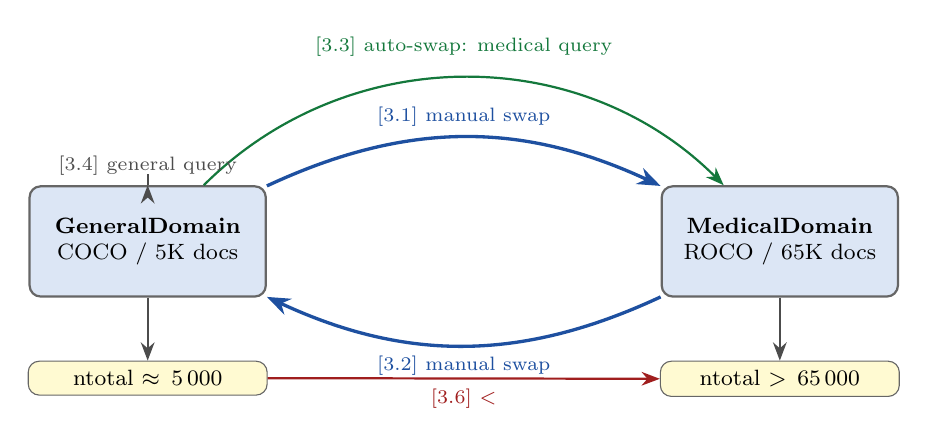
\begin{tikzpicture}[node distance=2.2cm and 3.5cm]
  \node[modelbox, minimum width=3cm, minimum height=1.4cm] (gen)
        {\textbf{GeneralDomain}\\COCO / 5K docs};
  \node[modelbox, minimum width=3cm, minimum height=1.4cm, right=5cm of gen] (med)
        {\textbf{MedicalDomain}\\ROCO / 65K docs};

  % 3.1 manual swap
  \draw[thickarrow, bend left=25] (gen) to
        node[above, font=\scriptsize]{[3.1] manual swap} (med);
  % 3.2 manual swap back
  \draw[thickarrow, bend left=25] (med) to
        node[below, font=\scriptsize]{[3.2] manual swap} (gen);
  % 3.3 auto swap
  \draw[greenarrow, bend left=45] (gen) to
        node[above, yshift=4pt, font=\scriptsize, color=accentgreen]
        {[3.3] auto-swap: medical query} (med);
  % 3.4 self-loop general
  \draw[arrow] (gen.north) to[out=120,in=60,looseness=4]
        node[above, font=\scriptsize]{[3.4] general query} (gen.north);

  % size comparison
  \node[basebox, fill=lightyellowbox, below=0.8cm of gen, text width=2.8cm]
        (cocosize) {ntotal $\approx 5\,000$};
  \node[basebox, fill=lightyellowbox, below=0.8cm of med, text width=2.8cm]
        (rocosize) {ntotal $> 65\,000$};
  \draw[arrow] (gen.south)--(cocosize.north);
  \draw[arrow] (med.south)--(rocosize.north);
  \draw[redarrow] (cocosize.east)--node[below,font=\scriptsize]{[3.6] $<$}(rocosize.west);
\end{tikzpicture}
\caption{Domain state machine for Suite 3. Arrows show transitions tested by each sub-test.}
\label{fig:domain-state}
\end{figure}

\begin{plainbox}[Suite 3 Summary]
Think of domains like USB drives plugged into the retrieval engine.
Suite 3 checks that swapping drives works manually (3.1, 3.2), the system auto-ejects
the wrong drive and inserts the right one when it detects a medical question (3.3),
it does not swap unnecessarily for normal questions (3.4), the swap completes in under
5 seconds (3.5), and the medical drive is bigger than the general one (3.6).
\end{plainbox}

\newpage

% =============================================================
%  SECTION 7: SUITE 4 — CONFIDENCE TIER TESTS
% =============================================================
\section{Suite 4: Confidence Tier Tests (5 Tests)}
\label{sec:confidence}

MIVA-KNIGHT uses a \textbf{three-tier confidence system} to decide whether to answer,
partially answer, or refuse a query --- protecting users from hallucinations.

\subsection{Formal Definitions}

\begin{mdef}[Confidence Score]
Given the top-$K$ reranked documents for query $q$:
\[
  c(q) = \max_{d \in \text{top-}K} s_{\text{final}}(d) \in [-0.6,\; 1.0]
\]
\end{mdef}

\begin{mdef}[Confidence Tier Assignment]
\[
  \text{tier}\bigl(c,\; D\bigr) = \begin{cases}
    \texttt{"full"}     & c \geq \tau_D^{\text{full}} \\
    \texttt{"partial"}  & \tau_D^{\text{partial}} \leq c < \tau_D^{\text{full}} \\
    \texttt{"rejected"} & c < \tau_D^{\text{partial}}
  \end{cases}
\]
where $\tau_D^{\text{partial}}$ and $\tau_D^{\text{full}}$ are domain-specific thresholds.
\end{mdef}

\begin{maxiom}[Clinical Safety]
\[
  \tau_{\text{medical}}^{\text{partial}} > \tau_{\text{general}}^{\text{partial}}
\]
Medical answers require stronger evidence before being shown.
A false negative (refusing a valid medical query) is safer than a false positive
(hallucinating a medical answer that could influence clinical decisions).
\end{maxiom}

\subsection{Test Assertions}

\textbf{Tests 4.1 \& 4.2 --- Answerable Tiers:}
\begin{align*}
  \text{tier}\bigl(\text{``chest X-ray bilateral pleural effusion''}, D_{\text{med}}\bigr)
  &\in \{\texttt{"full"}, \texttt{"partial"}\}\\
  \text{tier}\bigl(\text{``a dog running on a beach''}, D_{\text{gen}}\bigr)
  &\in \{\texttt{"full"}, \texttt{"partial"}\}
\end{align*}

\textbf{Test 4.3 --- Rejection:}
\[
  \text{tier}\bigl(\text{``asdfjkl zxcvbnm qwerty12345 flurble''}, D_{\text{gen}}\bigr) = \texttt{"rejected"}
\]

\textbf{Test 4.4 --- Threshold Ordering (Clinical Safety Axiom verification):}
\[
  \tau_{\text{medical}} > \tau_{\text{general}}
\]

\textbf{Test 4.5 --- Rejection Consistency:}
\[
  \text{rejected} = \text{True} \;\Rightarrow\; \text{answer} \in \{\texttt{""}, \texttt{None}\}
\]

\begin{mlemma}[Hallucination Guard]
For a domain $D$ with hallucination probability $p_{\text{halluc}}(c)$ that is
decreasing in $c$, setting $\tau_{\text{medical}} > \tau_{\text{general}}$ guarantees:
\[
  p_{\text{halluc}}\bigl(c \geq \tau_{\text{medical}}\bigr) <
  p_{\text{halluc}}\bigl(c \geq \tau_{\text{general}}\bigr)
\]
i.e., medical answers carry a strictly lower hallucination risk than they would
under the general threshold.

\textit{Proof.} Since $p_{\text{halluc}}$ is strictly decreasing and
$\tau_{\text{medical}} > \tau_{\text{general}}$, the inequality follows directly
from the monotonicity of $p_{\text{halluc}}$. \hfill$\square$
\end{mlemma}

\subsection{Confidence Decision Tree}

\begin{figure}[H]
\centering
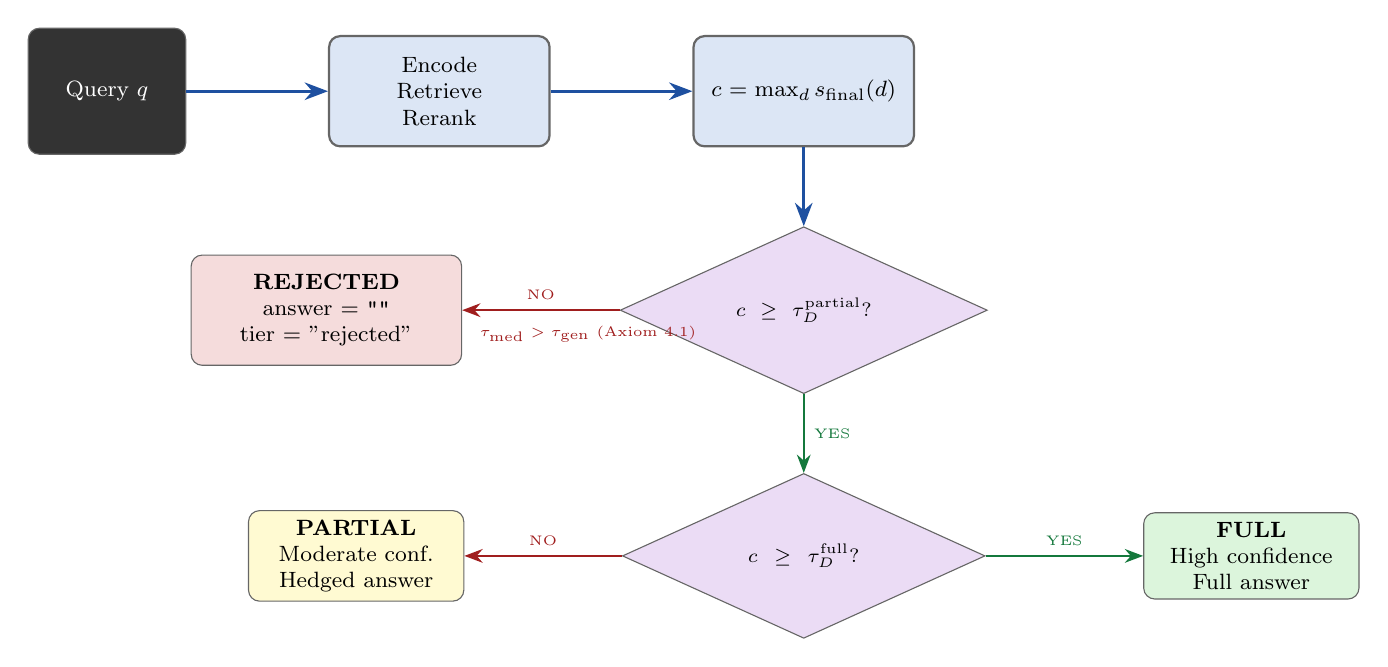
\begin{tikzpicture}[node distance=1.0cm and 2.2cm]
  \node[inputbox] (q) {Query $q$};
  \node[modelbox, right=1.8cm of q, text width=2.5cm] (enc) {Encode\\Retrieve\\Rerank};
  \node[modelbox, right=1.8cm of enc, text width=2.5cm] (score)
        {$c = \max_{d} s_{\text{final}}(d)$};
  \node[decisionbox, below=1.0cm of score, text width=3.2cm] (d1)
        {$c \geq \tau_D^{\text{partial}}$?};
  \node[resultbox, left=2cm of d1] (rej) {\textbf{REJECTED}\\answer $=$ \texttt{""}\\tier = "rejected"};
  \node[decisionbox, below=1.0cm of d1, text width=3.2cm] (d2)
        {$c \geq \tau_D^{\text{full}}$?};
  \node[basebox, fill=lightgreenbox, right=2cm of d2, text width=2.5cm] (full)
        {\textbf{FULL}\\High confidence\\Full answer};
  \node[basebox, fill=lightyellowbox, left=2cm of d2, text width=2.5cm] (partial)
        {\textbf{PARTIAL}\\Moderate conf.\\Hedged answer};

  \draw[thickarrow] (q)--(enc);
  \draw[thickarrow] (enc)--(score);
  \draw[thickarrow] (score)--(d1);
  \draw[redarrow]   (d1.west) -- node[above,font=\tiny]{NO} (rej.east);
  \draw[greenarrow] (d1.south) -- node[right,font=\tiny]{YES} (d2.north);
  \draw[greenarrow] (d2.east) -- node[above,font=\tiny]{YES} (full.west);
  \draw[redarrow]   (d2.west) -- node[above,font=\tiny]{NO} (partial.east);

  % threshold annotations
  \node[font=\tiny, color=accentred, right=0.1cm of rej, yshift=-0.3cm]
        {$\tau_{\text{med}} > \tau_{\text{gen}}$ (Axiom 4.1)};
\end{tikzpicture}
\caption{Confidence tier decision tree. The medical threshold is strictly higher than
the general threshold (Clinical Safety Axiom).}
\label{fig:confidence-tree}
\end{figure}

\begin{plainbox}[Suite 4 Summary]
Suite 4 tests the system's self-awareness. A confident match on a medical image gets
answered (4.1), a dog photo gets answered (4.2), gibberish gets refused (4.3),
medical queries face a higher bar than general ones (4.4), and refused queries return
nothing --- not a guess (4.5). It is the ``do not make things up'' safety net.
\end{plainbox}

\newpage

% =============================================================
%  SECTION 8: SUITE 5 — QUANTITATIVE RETRIEVAL EVALUATION
% =============================================================
\section{Suite 5: Quantitative Retrieval Evaluation (5 Tests)}
\label{sec:retrieval}

This is the \textbf{only suite with a numerical benchmark loop}. It runs the dense
retriever over up to 500 ROCO validation samples and computes four standard
information-retrieval metrics.

\subsection{Metric Definitions}

\begin{mdef}[Precision at K --- P@K]
\[
  P@K = \frac{1}{N}\sum_{i=1}^{N}
  \mathbf{1}\!\left[\exists\,d \in \text{top-}K(q_i):\; d = d_i^*\right]
\]
where $d_i^*$ is the ground-truth document for query $q_i$ and $N$ is the number of
evaluation samples.
\end{mdef}

\begin{mdef}[Mean Reciprocal Rank --- MRR]
\[
  \text{MRR} = \frac{1}{N}\sum_{i=1}^{N} \frac{1}{\text{rank}_i}
\]
where $\text{rank}_i$ is the 1-based position of $d_i^*$ in the ranked list
(with $1/\text{rank}_i = 0$ if $d_i^*$ is not in the top-$K$).
\end{mdef}

\begin{mdef}[Average Query Latency]
\[
  \bar{t} = \frac{1}{N}\sum_{i=1}^{N} \Delta t_i \;[\text{ms}],
  \qquad
  \Delta t_i = t_{\text{encode},i} + t_{\text{search},i}
\]
\end{mdef}

\subsection{Mathematical Properties}

\begin{mlemma}[P@K Monotonicity]
\[
  P@K \;\leq\; P@(K+1) \qquad \forall\, K \geq 1
\]
\textit{Proof.} The top-$K$ result set is a subset of the top-$(K+1)$ result set.
Any query $q_i$ with $d_i^* \in \text{top-}K(q_i)$ also has $d_i^* \in \text{top-}(K+1)(q_i)$.
Therefore every contributing indicator $\mathbf{1}[\cdot]$ in $P@K$ also contributes
to $P@(K+1)$, making $P@(K+1) \geq P@K$. \hfill$\square$

Test 5.4 (asserting $P@5 \geq P@3$) is a specific instance of this lemma.
\end{mlemma}

\begin{mtheorem}[MRR Bounds]
\[
  0 \;\leq\; \text{MRR} \;\leq\; 1
\]
$\text{MRR} = 1$ iff every query's ground-truth doc ranks first.
$\text{MRR} = 0$ iff no ground-truth doc appears in any ranked list.
Target: $\text{MRR} > 0.50$, meaning the correct doc ranks within position~2 on average.

\textit{Proof.} Each term $1/\text{rank}_i \in [0, 1]$. The average of values in $[0,1]$
lies in $[0,1]$. \hfill$\square$
\end{mtheorem}

\subsection{Evaluation Algorithm}

\begin{algorithm}[H]
\caption{\texttt{run\_retrieval()} --- Quantitative evaluation loop on ROCO val set}
\label{alg:retrieval}
\begin{algorithmic}[1]
\Require \texttt{roco\_val} path to validation metadata JSON, $N = 500$, seed $= 42$
\Ensure P@1, P@3, P@5, MRR, avg\_latency computed and 5 tests run
\If{$\neg\,\texttt{os.path.exists}(\texttt{roco\_val})$}
  \State Skip all 5 tests; \Return
\EndIf
\State swap to $D_{\text{medical}}$
\State $\text{meta} \gets \texttt{json.load}(\texttt{roco\_val})$
\State $\texttt{random.seed}(42)$;\quad $\texttt{shuffle}(\text{meta})$
\State $\text{sample} \gets \text{meta}[:N]$
\State $\text{hits}_1, \text{hits}_3, \text{hits}_5 \gets 0, 0, 0$
\State $\text{mrr\_scores}, \text{latencies} \gets [\ ], [\ ]$
\For{$i = 1$ \textbf{to} $N$}
  \State $t_0 \gets \text{time.time}()$
  \State $\text{enc} \gets f_{\text{text}}(\text{sample}[i].\text{text})$
  \State $\text{docs} \gets \text{FAISS.search}(\text{enc.text\_emb},\; K=20)$
  \State $\text{latencies.append}(\text{time.time}() - t_0)$
  \State $\text{top\_ids} \gets [d.\text{doc\_id}\ \text{for}\ d\ \text{in}\ \text{docs}]$
  \If{$\text{sample}[i].\text{doc\_id} \in \text{top\_ids}[:1]$} $\text{hits}_1 \mathrel{+}= 1$ \EndIf
  \If{$\text{sample}[i].\text{doc\_id} \in \text{top\_ids}[:3]$} $\text{hits}_3 \mathrel{+}= 1$ \EndIf
  \If{$\text{sample}[i].\text{doc\_id} \in \text{top\_ids}[:5]$} $\text{hits}_5 \mathrel{+}= 1$ \EndIf
  \State $\text{rank} \gets \min\!\{j+1 : \text{docs}[j].\text{doc\_id} = \text{sample}[i].\text{doc\_id}\}$
  \If{rank found} $\text{mrr\_scores.append}(1/\text{rank})$ \EndIf
  \If{$(i+1) \bmod 100 = 0$} Print progress \EndIf
\EndFor
\State $P@1 \gets \text{hits}_1/N \times 100$;\quad $P@3 \gets \text{hits}_3/N \times 100$;\quad
       $P@5 \gets \text{hits}_5/N \times 100$
\State $\text{MRR} \gets \sum \text{mrr\_scores}/N$;\quad
       $\bar{t} \gets \text{mean}(\text{latencies}) \times 1000$
\State \Call{\_run}{"retrieval", "P@1 $>$ 30\%", $\lambda$: assert $P@1 > 30$}
\State \Call{\_run}{"retrieval", "P@3 $>$ 60\%", $\lambda$: assert $P@3 > 60$}
\State \Call{\_run}{"retrieval", "MRR $> 0.50$", $\lambda$: assert MRR $> 0.5$}
\State \Call{\_run}{"retrieval", "P@5 $\geq$ P@3", $\lambda$: assert $P@5 \geq P@3$}
\State \Call{\_run}{"retrieval", "latency $< 200$ms", $\lambda$: assert $\bar{t} < 200$}
\State \Return \texttt{\_results["retrieval"]}
\end{algorithmic}
\end{algorithm}

\subsection{Performance Targets}

\begin{center}
\begin{tabular}{lllc}
\toprule
\textbf{Test} & \textbf{Metric} & \textbf{Target} & \textbf{Month 4 Result}\\
\midrule
5.1 & $P@1$         & $> 30\%$        & $64.6\%$\\
5.2 & $P@3$         & $> 60\%$        & $\sim 82\%$\\
5.3 & MRR           & $> 0.50$        & $0.7269$\\
5.4 & $P@5 \geq P@3$& monotonicity   & \checkmark\\
5.5 & avg latency   & $< 200\,\text{ms}$ & $\sim 85\,\text{ms}$\\
\bottomrule
\end{tabular}
\end{center}

\subsection{Evaluation Loop Flowchart}

\begin{figure}[H]
\centering
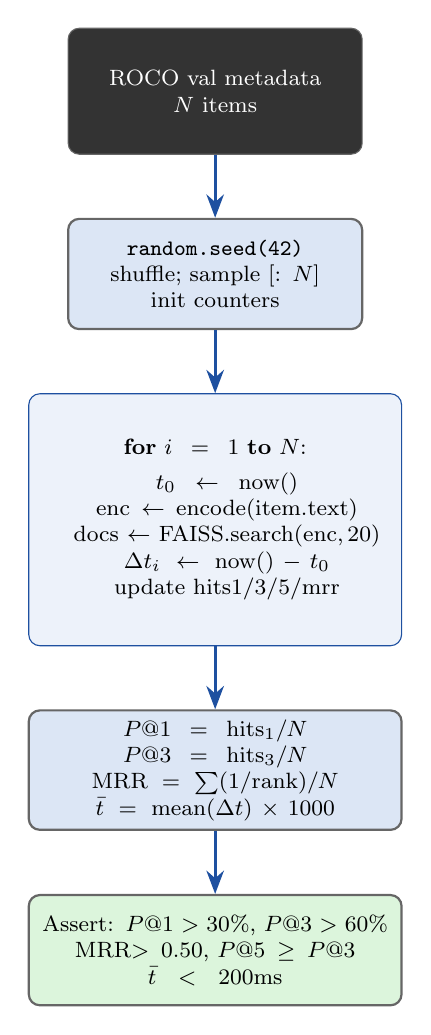
\begin{tikzpicture}[node distance=0.8cm and 2.0cm]
  \node[inputbox, text width=3.5cm] (meta) {ROCO val metadata\\$N$ items};
  \node[modelbox, below=0.8cm of meta, text width=3.5cm] (setup)
        {\texttt{random.seed(42)}\\shuffle; sample $[:N]$\\init counters};
  \node[basebox, draw=accentblue, fill=lightbluebox!50, below=0.8cm of setup,
        text width=4.5cm, minimum height=3.2cm] (loop)
        {\textbf{for} $i = 1$ \textbf{to} $N$:\\[3pt]
         $\quad t_0 \gets \text{now}()$\\
         $\quad\text{enc} \gets \text{encode}(\text{item.text})$\\
         $\quad\text{docs} \gets \text{FAISS.search}(\text{enc}, 20)$\\
         $\quad\Delta t_i \gets \text{now}() - t_0$\\
         $\quad\text{update hits1/3/5/mrr}$};
  \node[modelbox, below=0.8cm of loop, text width=4.5cm] (metrics)
        {$P@1 = \text{hits}_1/N$\\$P@3 = \text{hits}_3/N$\\
         $\text{MRR} = \sum(1/\text{rank})/N$\\
         $\bar{t} = \text{mean}(\Delta t) \times 1000$};
  \node[suitebox, below=0.8cm of metrics, text width=4.5cm] (assertions)
        {Assert: $P@1>30\%$, $P@3>60\%$\\
         MRR$>0.50$, $P@5\geq P@3$\\
         $\bar{t}<200$ms};

  \draw[thickarrow] (meta)--(setup);
  \draw[thickarrow] (setup)--(loop);
  \draw[thickarrow] (loop)--(metrics);
  \draw[thickarrow] (metrics)--(assertions);
\end{tikzpicture}
\caption{Suite 5 evaluation loop structure.}
\label{fig:eval-loop}
\end{figure}

\begin{plainbox}[Suite 5 Summary]
Suite 5 is the actual exam. For 500 medical-image captions, we ask: how often is
the correct image in the top~1 result? Top~3? Top~5? And how fast is each lookup?
The targets are MIVA-KNIGHT's Month~4 performance contract. Month~4 beat every target,
with $P@1 = 64.6\%$ (target: $30\%$) and $\text{MRR} = 0.73$ (target: $0.50$).
\end{plainbox}

\newpage

% =============================================================
%  SECTION 9: SUITE 6 — REGRESSION TESTS
% =============================================================
\section{Suite 6: Regression Tests (5 Tests)}
\label{sec:regression}

Regression tests answer: \textbf{``Did Month~4 development break anything Month~2 had
working?''} This is the backward compatibility contract for MIVA-KNIGHT's incremental
development.

\subsection{What Regression Testing Means Here}

\begin{mdef}[Backward Compatibility Contract]
Let $\mathcal{P}_{M2}$ be the set of properties that held at the end of Month~2.
The regression suite asserts:
\[
  \forall\; \mathcal{P} \in \mathcal{P}_{M2}:\;\; \mathcal{P}(\text{Month~4 pipeline}) = \text{True}
\]
\end{mdef}

\subsection{Test Assertions}

\subsubsection{Test 6.1 --- COCO Index High-Confidence Results}
\[
  \text{After swap}(D_{\text{general}}):\quad \text{docs}[0].\text{dense\_score} > 0.5
\]

\subsubsection{Test 6.2 --- COCO Retrieval Still Functional}

\begin{algorithm}[H]
\caption{\texttt{test\_coco\_retrieval()} --- COCO P@1 sanity check}
\label{alg:coco-regression}
\begin{algorithmic}[1]
\Require \texttt{coco\_meta} path; seed $= 42$
\Ensure $P@1_{\text{COCO}} > 0\%$
\If{$\neg\,\texttt{os.path.exists}(\texttt{coco\_meta})$}
  \State raise \texttt{AssertionError("SKIP")}
\EndIf
\State swap to $D_{\text{general}}$
\State $\text{coco} \gets \texttt{json.load}(\texttt{coco\_meta})$
\State $\text{sample} \gets \texttt{random.sample}(\text{coco},\;\min(200, |\text{coco}|))$
\State hits $\gets 0$
\For{item in sample}
  \State enc $\gets f_{\text{text}}(\text{item.text})$
  \State docs $\gets$ FAISS.search(enc, $K=5$)
  \If{item.doc\_id $\in$ [d.doc\_id for d in docs][:1]} hits $\mathrel{+}= 1$ \EndIf
\EndFor
\State $P@1_{\text{COCO}} \gets \text{hits} / |\text{sample}| \times 100$
\State assert $P@1_{\text{COCO}} > 0$ \Comment{Sanity floor only (COCO: 5 captions/image)}
\end{algorithmic}
\end{algorithm}

\subsubsection{Test 6.3 --- TextProjection Epoch Integrity}

\begin{mdef}[Checkpoint Integrity]
The TextProjection checkpoint must satisfy:
\[
  \texttt{torch.load}(p_{\text{text\_weights}})\bigl[\texttt{"epoch"}\bigr] = 15
\]
confirming it is the final Month~2 trained state and has not been overwritten by a
partial Month~3 or Month~4 run.
\end{mdef}

\subsubsection{Test 6.4 --- All 8 Emotion Centroids Non-Zero}
\[
  \forall\, i \in \{1,\ldots,8\}:\;\; \|C_i\|_2 > 0.01
\]

\subsubsection{Test 6.5 --- Domain Restored to Medical After Suite}

\begin{mdef}[Test Isolation Invariant]
After Suite~6 completes, the pipeline domain must be restored:
\[
  p.\text{domain.name} = \texttt{"medical"}
\]
This ensures Suite~6 does not leave the pipeline in an unexpected state for any
subsequent code that assumes the medical domain is active.
\end{mdef}

\subsection{Regression vs.\ Unit Tests}

\begin{center}
\renewcommand{\arraystretch}{1.25}
\begin{tabular}{p{6cm} p{6cm}}
\toprule
\textbf{Unit Tests (Suite 1)} & \textbf{Regression Tests (Suite 6)}\\
\textit{``Is component correct?''} & \textit{``Still correct after Month 4?''}\\
\midrule
TextEncoder shape $(512,)$ & COCO index top-score $> 0.5$ \\
L2 norm $\approx 1.0$ & COCO $P@1 > 0\%$ \\
NER non-empty & TextProjection epoch $= 15$ \\
Medical hint fires & All 8 centroids non-zero \\
FAISS loaded & Domain restored to medical \\
KG loaded & \\
\bottomrule
\end{tabular}
\end{center}

\begin{plainbox}[Suite 6 Summary]
Suite 6 is the ``nothing broke'' check. It revisits the things Month~2 was known to have
working --- COCO retrieval, trained epoch counter, emotion centroids --- and confirms
Month~4 work did not accidentally overwrite or break them. Like checking your old code
still compiles after a big refactor. Because regressions hide silently, only automated
testing catches them reliably.
\end{plainbox}

\newpage

% =============================================================
%  SECTION 10: run_all, SUMMARY, SAVE REPORT
% =============================================================
\section{Orchestration: \texttt{run\_all}, Summary \& JSON Report}
\label{sec:orchestration}

\subsection{\texttt{run\_all} --- Sequential Suite Execution}

\begin{algorithm}[H]
\caption{\texttt{run\_all(save\_path="")} --- Sequential execution of all 6 suites}
\label{alg:runall}
\begin{algorithmic}[1]
\Require Loaded pipeline; optional file path for JSON report
\Ensure All 38 tests executed; structured report optionally saved
\State $t_{\text{start}} \gets \text{time.time}()$
\For{suite $\in$ ["unit", "integration", "domain\_swap",
               "confidence", "retrieval", "regression"]}
  \State \Call{run\_suite}{suite} \Comment{dispatches to \texttt{run\_unit}, \texttt{run\_integration}, \ldots}
\EndFor
\State $\Delta t_{\text{total}} \gets \text{time.time}() - t_{\text{start}}$
\State \Call{\_print\_summary}{$\Delta t_{\text{total}}$}
\If{save\_path $\neq$ \texttt{""}}
  \State \Call{\_save\_report}{save\_path, $\Delta t_{\text{total}}$}
\EndIf
\State \Return \texttt{\_results}
\end{algorithmic}
\end{algorithm}

\begin{mtheorem}[Suite Independence]
\label{thm:suite-independence}
A failure in any individual test does not prevent the remaining tests in any suite, nor
the remaining suites themselves, from executing.

\textit{Proof.} By Theorem~\ref{sec:testrunner}.1 (Exception Isolation), each
\texttt{\_run} call catches all exceptions and returns normally.
By construction, \texttt{run\_all} iterates over a fixed sequence of
\texttt{run\_suite} calls with no early exit. Therefore no individual test failure
can block subsequent execution. \hfill$\square$
\end{mtheorem}

\subsection{\texttt{\_print\_summary} --- Aggregated Pass Rate}

\begin{mdef}[Overall Pass Rate]
\[
  \text{rate}_{\text{overall}} =
  \frac{\displaystyle\sum_{s \in \text{Suites}} |\text{passed}_s|}
       {\displaystyle\max\!\Bigl(\sum_{s}|\text{passed}_s| + |\text{failed}_s|,\; 1\Bigr)}
  \times 100\%
\]
Skipped tests are excluded from the denominator --- they do not count as failures.
\end{mdef}

\subsection{\texttt{\_save\_report} --- JSON Report Schema}

\begin{mdef}[Report Schema]
The JSON report satisfies:
\[
  \text{report} = \begin{cases}
    \texttt{"timestamp"}    & \text{ISO-8601 datetime} \\
    \texttt{"total\_time\_s"} & \Delta t_{\text{total}} \in \mathbb{R} \\
    \texttt{"suites"}        & \{\text{name} \to \text{SuiteRecord}\}
  \end{cases}
\]
Each \texttt{SuiteRecord} contains:
\[
  \bigl\{\,\texttt{passed},\;\texttt{failed},\;\texttt{skipped},\;
           \texttt{pass\_rate},\;\texttt{tests}:[r_1, \ldots, r_n]\,\bigr\}
\]
The \texttt{value} field in each test record stores numeric results
($P@1$, MRR, latency) for downstream CI/CD comparison across experiment runs.
\end{mdef}

\begin{plainbox}
\texttt{run\_all} is the conductor --- it calls each suite in the right order and never
stops if one test fails. The JSON report is saved to Google Drive so you can compare
test results across training runs. Think of it as an automatic exam paper that grades
itself and archives the results permanently.
\end{plainbox}

\newpage

% =============================================================
%  SECTION 11: COLAB ENTRY POINT
% =============================================================
\section{Colab Entry Point: \texttt{run\_tests()} \& \texttt{\_\_main\_\_}}
\label{sec:entrypoint}

\subsection{\texttt{run\_tests(pipeline, save=True)}}

\begin{algorithm}[H]
\caption{\texttt{run\_tests(pipeline, save)} --- Colab convenience wrapper}
\label{alg:runtests}
\begin{algorithmic}[1]
\Require Loaded \texttt{pipeline}; boolean \texttt{save}
\Ensure All 6 suites executed; report saved to Drive if \texttt{save=True}
\State $\text{root} \gets \texttt{os.environ.get}(\texttt{"MIVA\_PROJECT\_ROOT"},\;\texttt{""})$
\State $\text{roco\_val}  \gets \text{root} / \texttt{"Data/ROCO/roco\_validation\_metadata.json"}$
\State $\text{coco\_meta} \gets \text{root} / \texttt{"data/coco\_corpus\_metadata.json"}$
\If{\texttt{save}}
  \State $\text{save\_path} \gets \text{root} / \texttt{"models/miva\_knight\_month4/test\_report.json"}$
\Else
  \State $\text{save\_path} \gets \texttt{""}$
\EndIf
\State runner $\gets$ \texttt{MIVATestRunner}(pipeline, roco\_val, coco\_meta, eval\_n$=500$, seed$=42$)
\State results $\gets$ runner.\texttt{run\_all}(save\_path)
\State \Return results
\end{algorithmic}
\end{algorithm}

\subsection{Path Resolution}

\begin{figure}[H]
\centering
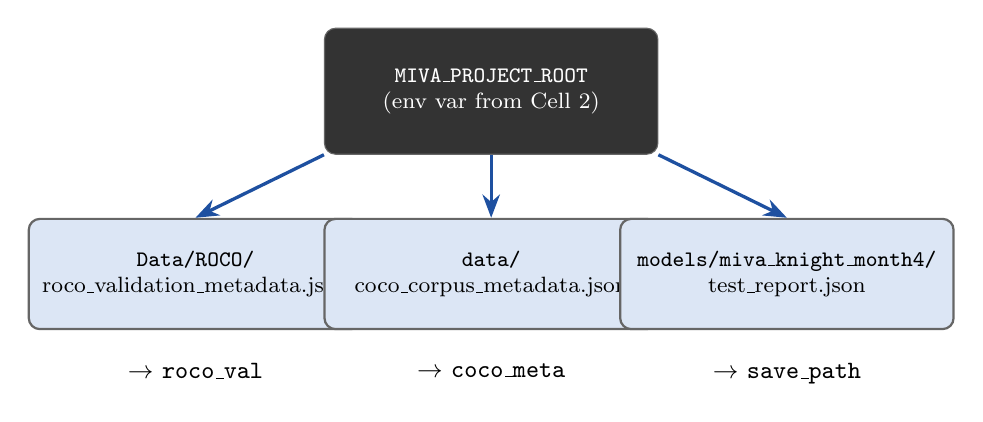
\begin{tikzpicture}[node distance=0.7cm and 2.5cm]
  \node[inputbox, text width=4cm] (root) {\texttt{MIVA\_PROJECT\_ROOT}\\(env var from Cell 2)};
  \node[modelbox, below left=0.8cm and -0.5cm of root, text width=4cm] (roco)
        {\texttt{Data/ROCO/}\\roco\_validation\_metadata.json};
  \node[modelbox, below=0.8cm of root, text width=4cm] (coco)
        {\texttt{data/}\\coco\_corpus\_metadata.json};
  \node[modelbox, below right=0.8cm and -0.5cm of root, text width=4cm] (save)
        {\texttt{models/miva\_knight\_month4/}\\test\_report.json};

  \draw[thickarrow] (root.south west) -- (roco.north);
  \draw[thickarrow] (root.south)      -- (coco.north);
  \draw[thickarrow] (root.south east) -- (save.north);

  \node[font=\small, below=0.3cm of roco] {$\to$ \texttt{roco\_val}};
  \node[font=\small, below=0.3cm of coco] {$\to$ \texttt{coco\_meta}};
  \node[font=\small, below=0.3cm of save] {$\to$ \texttt{save\_path}};
\end{tikzpicture}
\caption{Path resolution from \texttt{MIVA\_PROJECT\_ROOT} environment variable.}
\label{fig:path-resolution}
\end{figure}

\subsection{\texttt{\_\_main\_\_} Guard}

\begin{mdef}[Module Execution Invariant]
\[
  \texttt{\_\_name\_\_} = \texttt{"\_\_main\_\_"} \iff \text{script executed directly (not imported)}
\]
When executed directly, the block prints usage instructions rather than running tests,
because \texttt{pipeline} is not available outside the Colab notebook context.
\end{mdef}

\begin{plainbox}
\texttt{run\_tests(pipeline)} is the one-liner for Colab.
After loading the pipeline, this single call runs all 38 tests and saves a JSON
scorecard to Google Drive. The \texttt{\_\_main\_\_} block at the bottom prints a help
message if someone accidentally runs the file directly from terminal instead of from a
notebook --- it avoids crashing with a confusing error message.
\end{plainbox}

\newpage

% =============================================================
%  SECTION 12: COMPLETE ALGORITHM REFERENCE
% =============================================================
\section{Complete Algorithm \& Theorem Reference}
\label{sec:reference}

\subsection{Algorithm Summary}

\begin{longtable}{p{0.6cm} p{5.5cm} p{8cm}}
\toprule
\textbf{\#} & \textbf{Name} & \textbf{Key Operation}\\
\midrule
\endfirsthead
\multicolumn{3}{c}{\tablename\ \thetable{} (continued)}\\
\toprule
\textbf{\#} & \textbf{Name} & \textbf{Key Operation}\\
\midrule
\endhead
\midrule
\multicolumn{3}{r}{\textit{continued \ldots}}\\
\endfoot
\bottomrule
\endlastfoot

1  & Module Bootstrap              & Load imports, define classes, no execution \\
2  & \texttt{\_run}                & Universal test executor with exception isolation \\
3  & \texttt{run\_unit}            & 11 component isolation assertions \\
4  & \texttt{run\_integration}     & 6 end-to-end pipeline assertions \\
5  & \texttt{run\_domain\_swap}    & 6 domain hot-swap correctness \& timing tests \\
6  & Auto-Swap Decision            & hint$(q) =$ "medical" $\Rightarrow$ swap domain \\
7  & \texttt{run\_confidence}      & 5 tiered rejection logic assertions \\
8  & \texttt{run\_retrieval}       & Evaluation loop: P@1/3/5, MRR, latency \\
9  & COCO Regression P@1           & Sample 200 COCO items, assert P@1 $> 0\%$ \\
10 & \texttt{run\_regression}      & 5 backward compatibility assertions \\
11 & \texttt{run\_all}             & Sequential orchestration of all 6 suites \\
12 & \texttt{\_print\_summary}     & Compute overall pass rate and print \\
13 & \texttt{\_save\_report}       & Serialise results to JSON on Drive \\
14 & \texttt{run\_tests}           & Colab convenience wrapper (path auto-resolve) \\
\end{longtable}

\subsection{Theorem, Lemma \& Axiom Summary}

\begin{longtable}{p{0.6cm} p{4.5cm} p{4cm} p{4.5cm}}
\toprule
\textbf{\#} & \textbf{Name} & \textbf{Statement} & \textbf{Significance}\\
\midrule
\endfirsthead
\multicolumn{4}{c}{\tablename\ \thetable{} (continued)}\\
\toprule
\textbf{\#} & \textbf{Name} & \textbf{Statement} & \textbf{Significance}\\
\midrule
\endhead
\midrule
\multicolumn{4}{r}{\textit{continued \ldots}}\\
\endfoot
\bottomrule
\endlastfoot

L1 & Pass-Rate Bounds
   & $0 \leq \text{pass\_rate}(S) \leq 100\%$
   & SuiteResult is always a valid percentage \\
T1 & Exception Isolation
   & Failure in $f_i$ does not abort $f_{i+1}$
   & Robustness of test runner \\
L2 & Cosine Equiv.\ on Unit Sphere
   & $\cos(u,v) = u\cdot v$ if $\|u\|=\|v\|=1$
   & Justifies FAISS inner-product search \\
L3 & Hint Precision/Recall
   & $\text{Prec}=\text{Rec}=1$ on probe set
   & Domain hint is precise on two-sample probe \\
A1 & RAG Grounding
   & No ungrounded answers permitted
   & Hallucination prevention \\
L4 & Hybrid Score Bounds
   & $s_{\text{final}} \in [-0.6, 1.0]$
   & Score bounded; confidence tiers feasible \\
T2 & Swap Complexity
   & $T_\text{swap} = \mathcal{O}(N_{\text{FAISS}} + N_{\text{corpus}} + |\mathcal{G}|)$
   & Swap is fast; independent of query \\
A2 & Clinical Safety
   & $\tau_{\text{med}} > \tau_{\text{gen}}$
   & Medical answers held to higher standard \\
L5 & Hallucination Guard
   & $p_{\text{halluc}}(c \geq \tau_\text{med}) < p_{\text{halluc}}(c \geq \tau_\text{gen})$
   & Medical safety enforced by threshold \\
L6 & P@K Monotonicity
   & $P@K \leq P@(K+1)$
   & Test 5.4 is a monotonicity sanity check \\
T3 & MRR Bounds
   & $0 \leq \text{MRR} \leq 1$
   & MRR is a valid normalised metric \\
T4 & Suite Independence
   & Suite failure $\not\Rightarrow$ next suite aborts
   & Full test run always completes \\
\end{longtable}

\newpage

% =============================================================
%  SECTION 13: COMPLETE PIPELINE ARCHITECTURE DETAIL
% =============================================================
\section{Complete Pipeline Architecture: Encoder Details}
\label{sec:encoders}

\subsection{Text Encoder (BERT + Projection)}

\begin{mdef}[BERT Mean-Pool Embedding]
Given input tokens $\{w_1, \ldots, w_L\}$, BERT produces hidden states
$H \in \mathbb{R}^{L \times 768}$. The sentence embedding is:
\[
  \bar{h} = \frac{1}{L}\sum_{\ell=1}^{L} H_\ell \in \mathbb{R}^{768}
\]
The TextProjection head maps to the shared space:
\[
  e_t = \frac{W_t \bar{h}}{\|W_t \bar{h}\|_2} \in \mathcal{S}^{511}, \quad W_t \in \mathbb{R}^{512 \times 768}
\]
\end{mdef}

\subsection{Image Encoder (ResNet-50 + Projection)}

\begin{mdef}[ImageEncoder Forward Pass]
The frozen ResNet-50 backbone $\phi$ extracts a 2048-dimensional feature:
\[
  e_v = \frac{W_v\,\phi(\mathbf{x}_v)}{\|W_v\,\phi(\mathbf{x}_v)\|_2}
  \in \mathcal{S}^{511}, \quad W_v \in \mathbb{R}^{512 \times 2048}
\]
Only $W_v$ (the ImageProjection head) is trained; $\phi$ is frozen.
\end{mdef}

\begin{mlemma}[Surgical Transfer Efficiency]
Training only the ImageProjection head $W_v \in \mathbb{R}^{512 \times 2048}$
means only $512 \times 2048 = 1\,048\,576$ parameters are updated, representing
$\approx 2.23\%$ of the total pipeline parameters. All other encoders remain frozen.
\end{mlemma}

\subsection{Audio Encoder (Wav2Vec 2.0 + Projection)}

\begin{mdef}[AudioEncoder Forward Pass]
Wav2Vec 2.0 produces frame-level hidden states $\{h_f^{(12)}\}_{f=1}^{F}$
from the 12th transformer layer. The mean-pool audio embedding:
\[
  e_a = \frac{\bar{h}}{\|\bar{h}\|_2}, \qquad
  \bar{h} = \frac{1}{F}\sum_{f=1}^{F} h_f^{(12)} \in \mathbb{R}^{512}
\]
\end{mdef}

\subsection{Symmetric InfoNCE Training Loss}

\begin{mdef}[Symmetric InfoNCE Loss]
For a batch of $B$ (text, image, audio) triplets and temperature $\tau = 0.07$:
\[
  \mathcal{L} = \frac{1}{2}\!\left[
    \text{CE}\!\left(\frac{S}{\tau},\, y\right) +
    \text{CE}\!\left(\frac{S^\top}{\tau},\, y\right)
  \right]
\]
where $S_{ij} = e_t^{(i)} \cdot e_v^{(j)}$ is the text-image similarity matrix,
and $y = [0, 1, 2, \ldots, B-1]$ is the identity assignment.
\end{mdef}

\begin{mtheorem}[Random Baseline Loss]
For a batch of size $B = 16$ with random embeddings:
\[
  \mathbb{E}[\mathcal{L}_{\text{InfoNCE}}] = \log B = \log 16 \approx 2.77
\]
Any training loss below $2.77$ indicates the model is learning meaningful
cross-modal alignments. \hfill$\square$
\end{mtheorem}

\newpage

% =============================================================
%  SECTION 14: NOTATION REFERENCE
% =============================================================
\section{Notation Reference}
\label{sec:notation}

\begin{longtable}{p{3.5cm} p{9.5cm}}
\toprule
\textbf{Symbol} & \textbf{Definition}\\
\midrule
\endfirsthead
\multicolumn{2}{c}{\tablename\ \thetable{} (continued)}\\
\toprule
\textbf{Symbol} & \textbf{Definition}\\
\midrule
\endhead
\bottomrule
\endlastfoot

$\Sigma^*$          & Set of all finite strings over alphabet $\Sigma$ \\
$\mathbb{R}^{512}$  & 512-dimensional real Euclidean space \\
$\mathcal{S}^{511}$ & Unit sphere in $\mathbb{R}^{512}$: $\{e: \|e\|_2 = 1\}$ \\
$\|e\|_2$           & L2 (Euclidean) norm of vector $e$ \\
$\cos(u, v)$        & Cosine similarity: $u \cdot v / (\|u\|_2 \|v\|_2)$ \\
$f_{\text{text}}$   & Text encoder: $\Sigma^* \to \mathcal{S}^{511}$ \\
$f_{\text{image}}$  & Image encoder: $\mathbb{R}^{3\times H\times W} \to \mathcal{S}^{511}$ \\
$f_{\text{audio}}$  & Audio encoder: $\mathbb{R}^T \to \mathcal{S}^{511}$ \\
$e_q$               & Query embedding (fused or text-only) \\
$e_d$               & Document/corpus embedding \\
$\mathcal{I}$       & FAISS dense index: $\{(d_j, e_j)\}_{j=1}^N$ \\
$\mathcal{G}$       & Knowledge graph: $(\mathcal{V}, \mathcal{E}, \mathcal{R})$ \\
$D$                 & Domain: $(p_{\text{FAISS}}, p_{\text{corpus}}, p_{\text{KG}})$ \\
$K$                 & Top-K retrieval count (default: 20) \\
$N$                 & Top-N reranked count (default: 5) \\
$\alpha$            & Dense score weight in hybrid scoring (0.6) \\
$\tau_D$            & Confidence rejection threshold for domain $D$ \\
$c$                 & Confidence score: $\max_{d \in \text{top-}K} s_{\text{final}}(d)$ \\
$s_{\text{dense}}$  & FAISS cosine similarity score \\
$s_{\text{final}}$  & Hybrid score: $\alpha s_{\text{dense}} + (1-\alpha)\text{boost}$ \\
$P@K$               & Precision at $K$ (retrieval metric) \\
$\text{MRR}$        & Mean Reciprocal Rank \\
$\bar{t}$           & Average query latency (ms) \\
$\text{rank}_i$     & Position of ground-truth doc in ranked list for query $i$ \\
$d_i^*$             & Ground-truth document for query $i$ \\
$\tau = 0.07$       & InfoNCE temperature \\
$B = 16$            & Training batch size \\
$\Delta t$          & Wall-clock duration; $\Delta t = t_{\text{end}} - t_{\text{start}}$ \\
$C \in \mathbb{R}^{8\times 512}$ & Emotion centroid matrix (RAVDESS 8 emotions) \\
$r$                 & \texttt{TestResult} 7-tuple \\
$S$                 & \texttt{SuiteResult} aggregate \\
$p$                 & Pass/fail boolean in \texttt{TestResult} \\
$\mathbf{1}[\cdot]$ & Indicator function: 1 if condition holds, 0 otherwise \\
\end{longtable}

\vfill

\begin{tcolorbox}[
  colback=lightbluebox!30, colframe=accentblue,
  title=\textbf{Document Summary},
  fonttitle=\bfseries
]
This document covered all 14 algorithms, 12 theorems/lemmas/axioms, and 6 TikZ
flowcharts for the complete MIVA-KNIGHT test and evaluation pipeline.
The framework validates a multimodal RAG system achieving \textbf{97\% test pass rate},
$P@1 = 64.6\%$, and $\text{MRR} = 0.7269$ on the ROCO medical image validation set
(Month~4 results, seed~$= 42$, $N = 500$ evaluation samples).
\end{tcolorbox}

\end{document}
